% !TeX program = xelatex
\documentclass[aspectratio=169,11pt]{beamer}

% -------------------------------------------------
% Packages
% -------------------------------------------------
\usepackage{kotex}
\usepackage{fontspec}
\usepackage{amsmath,amssymb,bm,mathtools}
\usepackage{booktabs,array}
\usepackage{xcolor}
\usepackage{colortbl}
\usepackage{tikz}
\usepackage{pifont}
\usetikzlibrary{positioning,arrows.meta,calc,fit,decorations.pathreplacing,backgrounds,matrix}
\usepackage[most]{tcolorbox}
\usepackage{listings}
\usepackage{adjustbox}

% -------------------------------------------------
% Colors (same as the notes)
% -------------------------------------------------
\definecolor{deepblue}{RGB}{34,71,120}
\definecolor{softblue}{RGB}{239,246,253}
\definecolor{softgray}{RGB}{246,247,249}
\definecolor{softgreen}{RGB}{239,249,242}
\definecolor{softyellow}{RGB}{255,249,229}
\definecolor{codegray}{RGB}{248,248,248}
% colors of the graph figures
\definecolor{fwd}{RGB}{31,100,180}      % the original (forward) graph
\definecolor{der}{RGB}{214,110,0}       % the derivative graph
\definecolor{lossc}{RGB}{120,60,160}    % residual and loss
\definecolor{bwd}{RGB}{200,30,40}       % backward pass

% -------------------------------------------------
% Beamer look (same as the CNN slides)
% -------------------------------------------------
\usetheme{default}
\usefonttheme[onlymath]{serif}
\setbeamertemplate{navigation symbols}{}
\setbeamersize{text margin left=8mm,text margin right=8mm}
\setbeamercolor{structure}{fg=deepblue}
\setbeamercolor{frametitle}{fg=deepblue}
\setbeamercolor{title}{fg=deepblue}
\setbeamerfont{frametitle}{size=\large,series=\bfseries}
\setbeamertemplate{itemize items}[circle]
\setbeamertemplate{enumerate items}[default]
\setbeamertemplate{frametitle}{%
  \vskip3mm
  {\usebeamerfont{frametitle}\usebeamercolor[fg]{frametitle}\insertframetitle\par}%
  \vskip1mm
  {\color{deepblue!45}\hrule height 0.6pt}%
  \vskip1mm}
\setbeamertemplate{footline}{%
  \hbox to\paperwidth{%
    \hspace*{8mm}{\color{black!45}\scriptsize 물리 정보 신경망 (PINN)\ifx\insertsectionhead\empty\else\ \ $\cdot$\ \ \insertsectionhead\fi}%
    \hfill{\color{black!45}\scriptsize\insertframenumber\,/\,\inserttotalframenumber}\hspace*{8mm}}%
  \vskip2.5mm}
\setbeamertemplate{title page}{%
  \vfill
  \begin{center}
  {\color{deepblue}\Huge\bfseries\inserttitle\par}
  \vskip3mm
  {\color{deepblue!60}\rule{9cm}{0.8pt}\par}
  \vskip3mm
  {\large\insertsubtitle\par}
  \vskip8mm
  {\normalsize\insertdate\par}
  \end{center}
  \vfill}
\AtBeginSection[]{%
  \begin{frame}
  \vfill
  \centering
  {\color{deepblue!55}\Large\bfseries \insertsectionnumber\par}
  \vskip2mm
  {\color{deepblue}\LARGE\bfseries\insertsectionhead\par}
  \vskip3mm
  {\color{deepblue!50}\rule{7cm}{0.8pt}\par}
  \vfill
  \end{frame}}
\setlength{\leftmargini}{1.2em}
\setlength{\leftmarginii}{1.1em}

% -------------------------------------------------
% Boxes (same colors as the notes)
% -------------------------------------------------
\newtcolorbox{keybox}[1][]{colback=softblue,colframe=deepblue,boxrule=0.7pt,arc=2mm,
  title=#1,fonttitle=\bfseries\small,left=2mm,right=2mm,top=1mm,bottom=1mm,
  toptitle=0.5mm,bottomtitle=0.5mm}
\newtcolorbox{thinkbox}[1][]{colback=softyellow,colframe=orange!70!black,boxrule=0.6pt,arc=2mm,
  title=#1,fonttitle=\bfseries\small,left=2mm,right=2mm,top=1mm,bottom=1mm,
  toptitle=0.5mm,bottomtitle=0.5mm}
\newtcolorbox{remarkbox}[1][]{colback=softgray,colframe=black!45,boxrule=0.5pt,arc=2mm,
  title=#1,fonttitle=\bfseries\small,left=2mm,right=2mm,top=1mm,bottom=1mm,
  toptitle=0.5mm,bottomtitle=0.5mm}

% -------------------------------------------------
% Code style
% -------------------------------------------------
\lstdefinestyle{pythonstyle}{
  language=Python,
  backgroundcolor=\color{codegray},
  basicstyle=\ttfamily\scriptsize,
  keywordstyle=\bfseries\color{deepblue},
  commentstyle=\itshape\color{black!55},
  stringstyle=\color{black!75},
  numbers=none,
  frame=single,
  rulecolor=\color{black!25},
  breaklines=true,
  showstringspaces=false,
  tabsize=4,
  columns=fullflexible,
  keepspaces=true,
  aboveskip=1mm,
  belowskip=1mm
}
\lstset{style=pythonstyle}

% -------------------------------------------------
% Math commands (same as the notes)
% -------------------------------------------------
\newcommand{\R}{\mathbb{R}}
\newcommand{\vect}[1]{\bm{#1}}
\newcommand{\T}{^{\mathsf T}}
\newcommand{\loss}{\mathcal{L}}
\newcommand{\pd}[2]{\frac{\partial #1}{\partial #2}}

% TikZ styles shared by the graph figures (same as the notes)
\tikzset{
  >=Latex,
  val/.style={draw=#1!80!black,fill=#1!10,rounded corners=3pt,align=center,font=\small,inner sep=3pt,minimum height=9mm},
  par/.style={draw=black!60,fill=black!6,font=\small,inner sep=2.5pt,minimum size=6mm},
  eg/.style={->,thick,#1!80!black},
  elab/.style={font=\scriptsize,fill=white,inner sep=1pt},
  box/.style={draw=#1!70!black,fill=#1!8,rounded corners=3pt,align=center,font=\small,inner sep=4pt},
  sval/.style={draw=#1!80!black,fill=#1!10,rounded corners=3pt,align=center,font=\small,inner sep=3pt,minimum height=7mm},
  st/.style={draw=#1!70!black,fill=#1!8,rounded corners=3pt,align=center,font=\small,text width=26mm,minimum height=24mm,inner sep=2pt},
}

% one-line caption under a figure
\newcommand{\figcap}[1]{\par\vskip1mm{\centering\footnotesize\color{black!70}#1\par}}

\title{물리 정보 신경망 (PINN)}
\subtitle{입력에 대한 미분 $\cdot$ 미분 그래프 $\cdot$ residual loss $\cdot$ 순문제와 역문제}
\date{딥러닝개론및연습 $\cdot$ 2026년 2학기}

\begin{document}

% =================================================
\begin{frame}[plain]
\titlepage
\end{frame}

\begin{frame}{이번 단원의 핵심 질문}
\begin{keybox}[이번 단원의 핵심 질문]
\begin{itemize}
\item 지금까지 신경망은 \textbf{정답이 붙은 데이터}에서 배웠다 (지도학습)
\item 물리와 공학에서는 데이터는 적어도 \textbf{법칙}, 즉 미분방정식은 알고 있는 경우가 많다
\item 신경망에게 데이터 대신 \textbf{방정식}을 가르칠 수는 없을까?
\item 그때 PyTorch 안에서는 정확히 무슨 일이 일어나는가?
\end{itemize}
\end{keybox}
\vskip2mm
``자동미분, loss, \texttt{optimizer.step()}''으로 뭉뚱그려 두었던 과정을 이번에는 계산 그래프의 노드 하나하나까지 따라간다.
\end{frame}

\begin{frame}{학습목표}
\begin{enumerate}
\item 신경망의 출력을 \textbf{입력}으로 미분하는 것과 가중치로 미분하는 것의 차이
\item 작은 신경망에서 $u$, $u_x$, $u_{xx}$의 계산 그래프: 미분 그래프는 원래 그래프의 노드를 재료로 쓰는 새 그래프
\item residual loss의 gradient가 \textbf{여러 경로를 거쳐 더해져} 가중치에 도착함을 손으로 계산
\item \texttt{torch.autograd.grad}의 \texttt{create\_graph}, \texttt{grad\_outputs}의 역할
\item 1차원 Poisson 방정식과 열 방정식을 PINN으로 풀고 오차 측정
\item 미지의 계수를 데이터와 방정식으로 함께 찾는 \textbf{역문제}
\item PINN의 한계 (높은 주파수, loss 균형, 계산 비용)와 고전적인 수치해법과의 비교
\end{enumerate}
\end{frame}

\begin{frame}{목차}
\small
\tableofcontents
\end{frame}

% =================================================
\section{PINN이란 무엇인가}
% =================================================

\begin{frame}{정답 데이터가 하나도 없는 문제}
지금까지: 입력과 정답의 쌍 $(x_i,y_i)$로 $u_\theta(x_i)\approx y_i$가 되도록 $\theta$를 학습.

\vskip2mm
이제 다음 \textbf{경계값 문제}를 풀자 (1차원 \textbf{Poisson 방정식}).
\[
-u''(x)=f(x)\quad (0<x<1),\qquad u(0)=0,\quad u(1)=0.
\]
$f(x)=\pi^2\sin(\pi x)$이면 정확한 해는 $u^*(x)=\sin(\pi x)$.

\vskip2mm
\begin{columns}[T,onlytextwidth]
\begin{column}{0.48\textwidth}
\begin{remarkbox}[없는 것]
$u^*$의 값 (정답 데이터)
\end{remarkbox}
\end{column}
\begin{column}{0.48\textwidth}
\begin{keybox}[아는 것: 해가 만족할 조건]
\begin{itemize}
\item 내부의 모든 점에서 $-u''(x)-f(x)=0$
\item 경계에서 $u(0)=0$, $u(1)=0$
\end{itemize}
\end{keybox}
\end{column}
\end{columns}
\end{frame}

\begin{frame}{residual과 PINN의 loss}
신경망 $u_\theta$가 조건을 어기는 정도를 loss로 삼는다. 방정식을 어기는 정도
\[
r_\theta(x)=-u_\theta''(x)-f(x)
\]
를 \textbf{residual} (잔차)이라 한다. 내부에서 고른 \textbf{collocation point} $x_1,\dots,x_N$에서
\[
\loss(\theta)=\underbrace{\frac1N\sum_{i=1}^N r_\theta(x_i)^2}_{\text{방정식 (PDE) 항}}
+\lambda\,\underbrace{\frac12\Big(u_\theta(0)^2+u_\theta(1)^2\Big)}_{\text{경계조건 항}}
\]
을 최소화한다. 이것이 \textbf{Physics-Informed Neural Network (PINN)}의 전부이다.

\vskip2mm
\begin{keybox}
훈련 데이터는 어디에? collocation point가 그 역할을 한다. 방정식을 만족시키고 싶은 점을 \textbf{원하는 만큼} 만들 수 있다.
\end{keybox}
\end{frame}

\begin{frame}{지도학습과 PINN: 바뀐 것은 loss를 만드는 방법뿐}
\centering
\begin{adjustbox}{max width=\linewidth,max totalheight=5.6cm}
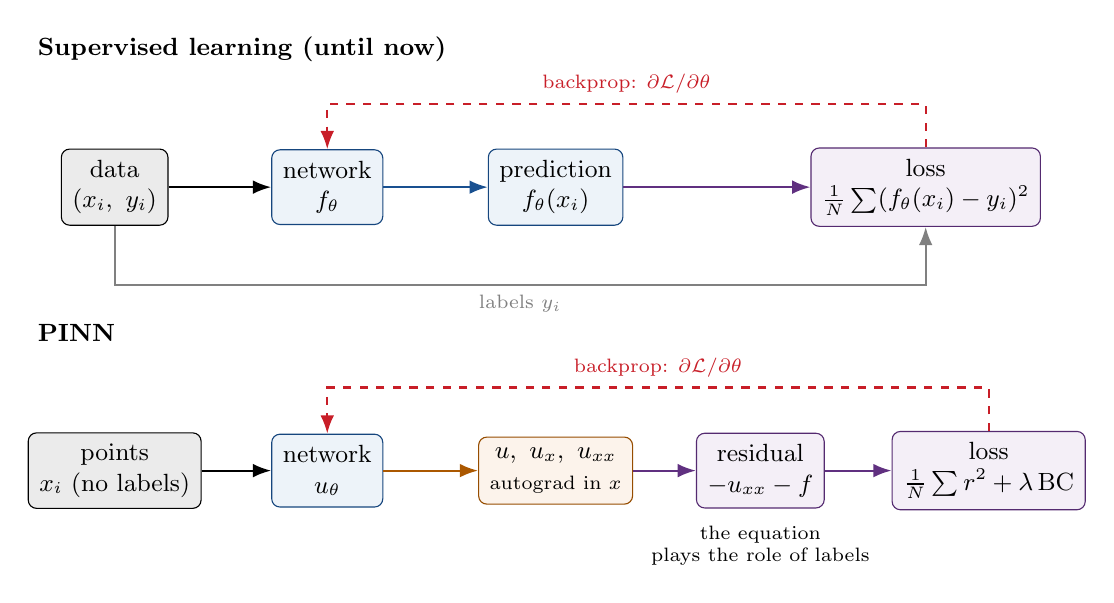
\begin{tikzpicture}[node distance=5mm]
\node[font=\small\bfseries,anchor=west] at (-0.2,1.75) {Supervised learning (until now)};
\node[box=black] (d1) at (0.9,0) {data\\$(x_i,\ y_i)$};
\node[box=fwd]   (n1) at (3.6,0) {network\\$f_\theta$};
\node[box=fwd]   (p1) at (6.5,0) {prediction\\$f_\theta(x_i)$};
\node[box=lossc] (l1) at (11.2,0) {loss\\$\frac1N\sum(f_\theta(x_i)-y_i)^2$};
\draw[eg=black] (d1) -- (n1); \draw[eg=fwd] (n1) -- (p1); \draw[eg=lossc] (p1) -- (l1);
\draw[->,thick,black!50]   (d1.south) |- ++(0,-0.75) -| node[pos=0.25,below,font=\scriptsize] {labels $y_i$} (l1.south);
\draw[->,thick,dashed,bwd] (l1.north) -- ++(0,0.55)  -| node[pos=0.25,above,font=\scriptsize] {backprop: $\partial\loss/\partial\theta$} (n1.north);
\begin{scope}[yshift=-3.6cm]
\node[font=\small\bfseries,anchor=west] at (-0.2,1.75) {PINN};
\node[box=black] (d2) at (0.9,0) {points\\$x_i$ (no labels)};
\node[box=fwd]   (n2) at (3.6,0) {network\\$u_\theta$};
\node[box=der]   (p2) at (6.5,0) {$u,\ u_x,\ u_{xx}$\\{\scriptsize autograd in $x$}};
\node[box=lossc] (r2) at (9.1,0) {residual\\$-u_{xx}-f$};
\node[box=lossc] (l2) at (12.0,0) {loss\\$\frac1N\sum r^2+\lambda\,\mathrm{BC}$};
\draw[eg=black] (d2) -- (n2); \draw[eg=der] (n2) -- (p2); \draw[eg=lossc] (p2) -- (r2); \draw[eg=lossc] (r2) -- (l2);
\node[font=\scriptsize,below=1mm of r2,align=center] {the equation\\plays the role of labels};
\draw[->,thick,dashed,bwd] (l2.north) -- ++(0,0.55) -| node[pos=0.25,above,font=\scriptsize] {backprop: $\partial\loss/\partial\theta$} (n2.north);
\end{scope}
\end{tikzpicture}
\end{adjustbox}
\figcap{정답 대신 방정식이 신경망을 평가한다. 학습 (역전파와 optimizer)은 지금까지와 똑같다.}
\end{frame}

\begin{frame}{방정식이 주는 정보 (\texttt{data\_vs\_physics.py})}
같은 신경망을 세 가지 loss로 학습: (A) $[0,0.4]$의 측정값 $8$개만, (B) 방정식만, (C) 둘 다.
\vskip1mm
\centering
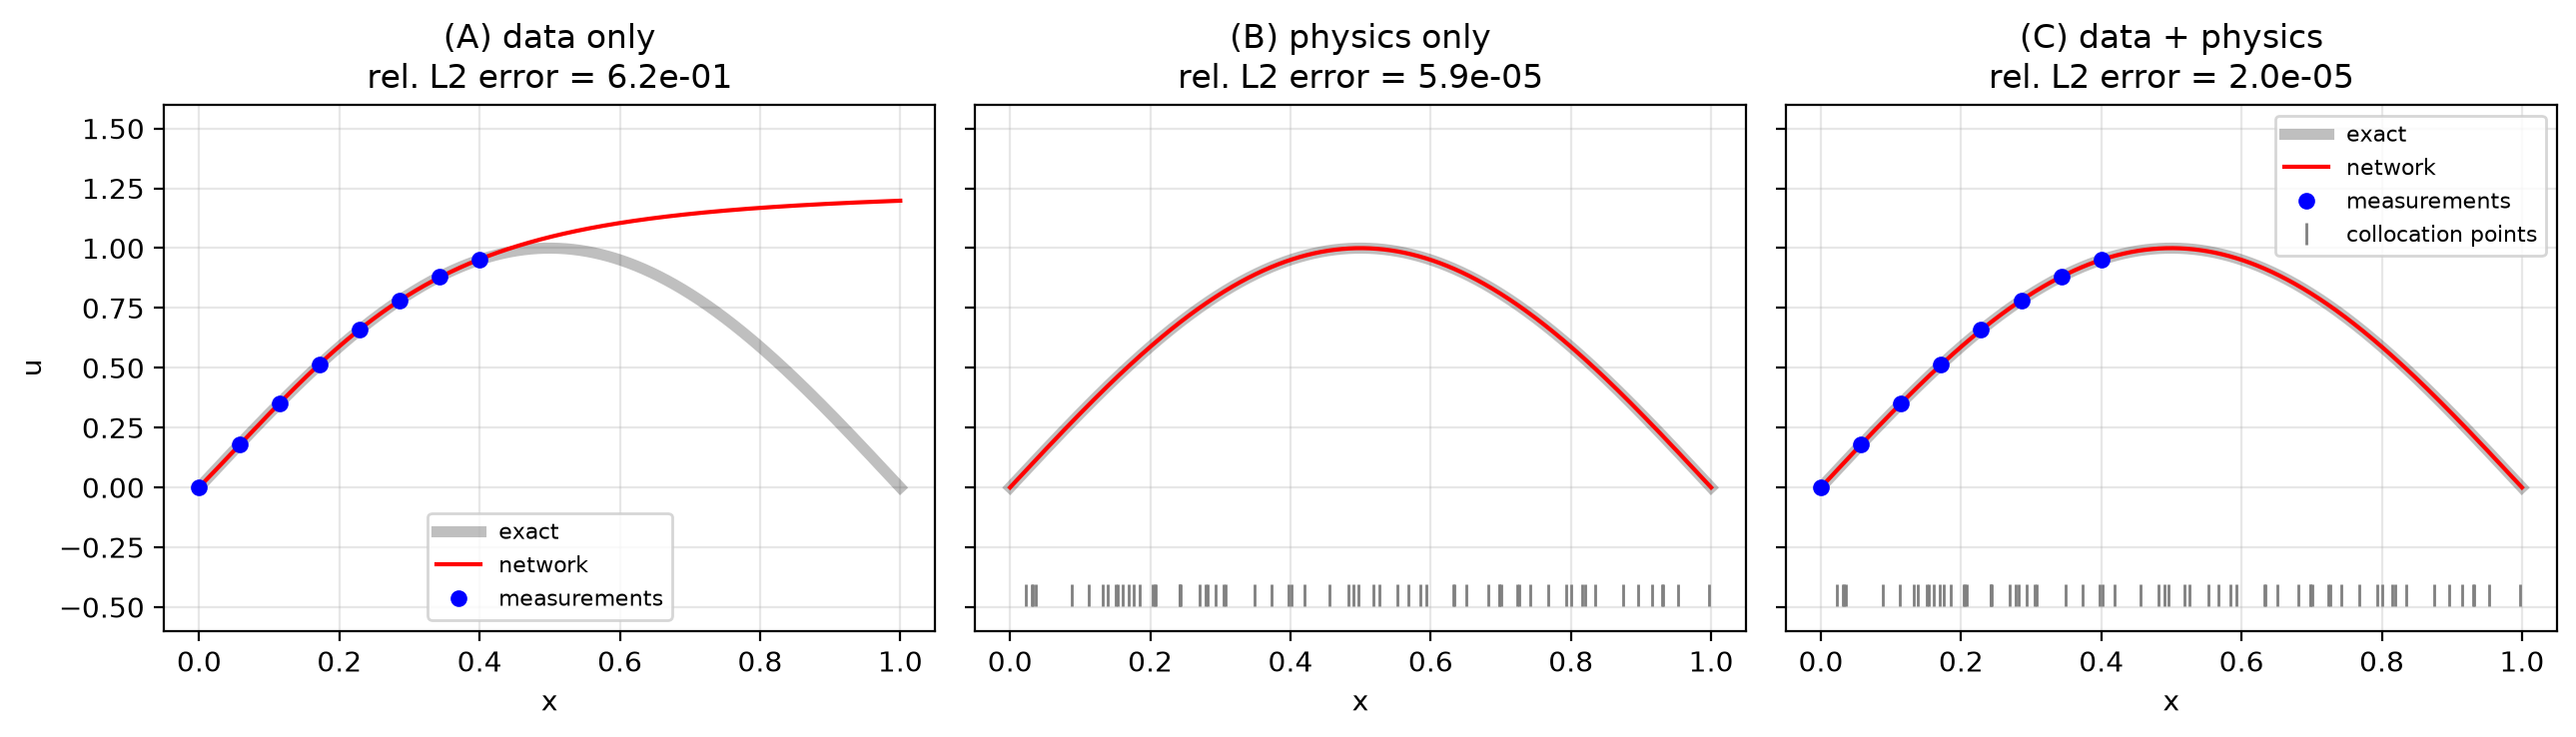
\includegraphics[width=\linewidth]{figures/data_vs_physics.png}
\figcap{측정값이 $[0,0.4]$에만 있을 때. (A)는 측정값이 없는 곳에서 엉뚱한 곡선을 그린다. (B)는 측정값 없이도 해를 찾는다.}
\end{frame}

\begin{frame}{오차를 재는 방법: 상대 $L^2$ 오차}
시험점 $z_1,\dots,z_M$에서
\[
\frac{\|u_\theta-u^*\|_2}{\|u^*\|_2}
=\left(\frac{\sum_{m=1}^M\big(u_\theta(z_m)-u^*(z_m)\big)^2}{\sum_{m=1}^M u^*(z_m)^2}\right)^{1/2}
\]
($\int(u_\theta-u^*)^2$과 $\int(u^*)^2$을 점들의 합으로 근사한 비의 제곱근). 1차원에서는 $[0,1]$의 등간격 $M=1001$개 점.

\vskip1mm
\begin{center}
\small
\begin{tabular}{@{}lll@{}}
\toprule
& 상대오차 & 이유 \\
\midrule
(A) 데이터만 & $0.62$ & $x>0.4$에서 해를 정할 정보가 loss에 없다 \\
(B) 방정식만 & $5.9\times10^{-5}$ & 해가 유일하므로 loss가 $0$인 함수는 $u^*$뿐 \\
(C) 데이터 + 방정식 & $2.0\times10^{-5}$ & 방정식은 빈 영역을, 측정값은 방정식에 없는 정보를 \\
\bottomrule
\end{tabular}
\end{center}

\figcap{PINN의 역사: Lagaris, Likas, Fotiadis (1998)는 $u_\theta''$의 식을 손으로 유도. Raissi, Perdikaris, Karniadakis (2019)가 \textbf{자동미분}으로 일반화.}
\end{frame}

% =================================================
\section{신경망은 입력의 함수이다}
% =================================================

\begin{frame}{두 종류의 미분}
\centering
\begin{adjustbox}{max width=0.85\linewidth,max totalheight=3.3cm}
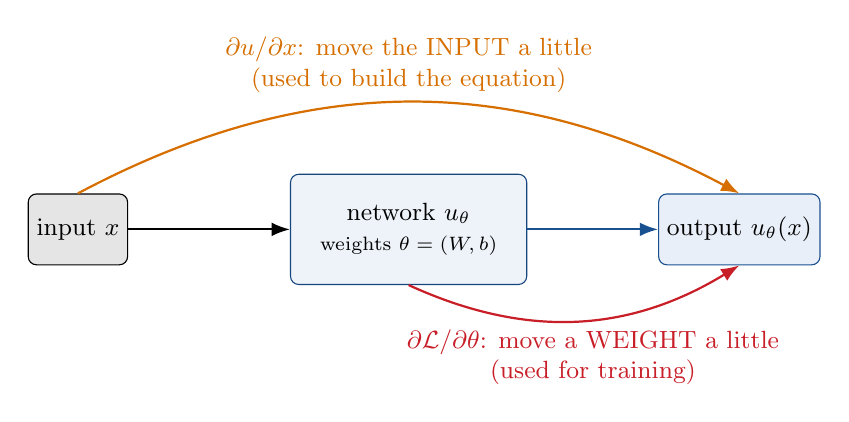
\begin{tikzpicture}
\node[box=fwd,minimum width=30mm,minimum height=14mm] (net) at (0,0) {network $u_\theta$\\{\scriptsize weights $\theta=(W,b)$}};
\node[val=black] (x) at (-4.2,0) {input $x$};
\node[val=fwd] (u) at (4.2,0) {output $u_\theta(x)$};
\draw[eg=black] (x) -- (net); \draw[eg=fwd] (net) -- (u);
\draw[->,thick,der,bend left=28] (x.north) to node[above,font=\small,align=center] {$\partial u/\partial x$: move the INPUT a little\\(used to build the equation)} (u.north);
\draw[->,thick,bwd,bend right=28] (net.south) to node[below,font=\small,align=center,pos=0.55] {$\partial \loss/\partial\theta$: move a WEIGHT a little\\(used for training)} (u.south);
\end{tikzpicture}
\end{adjustbox}

\vskip2mm
\small
\begin{tabular}{@{}lll@{}}
\toprule
& $\partial\loss/\partial\theta$ & $\partial u_\theta/\partial x$ \\
\midrule
무엇을 움직이는가 & 가중치 $\theta$ & 입력 $x$ (가중치는 고정) \\
어디에 쓰는가 & 경사하강법으로 학습 & 방정식 (residual)을 만들 때 \\
PyTorch & \texttt{loss.backward()} & \texttt{torch.autograd.grad(u, x, ...)} \\
결과의 모양 & 가중치와 같은 모양 & 입력과 같은 모양 $(N,1)$ \\
\bottomrule
\end{tabular}
\figcap{둘 다 계산 그래프 위의 연쇄법칙. 자동미분에게 입력 $x$는 가중치와 같은 \textbf{잎 (leaf) 노드}이다.}
\end{frame}

\begin{frame}{활성화 함수는 매끄러워야 한다: tanh와 ReLU}
\begin{columns}[c,onlytextwidth]
\begin{column}{0.40\textwidth}
\footnotesize
은닉층이 하나이면
\[
u_\theta''(x)=\sum_j v_j\,w_j^2\,\sigma''(w_jx+b_j).
\]
\begin{itemize}
\item $\tanh\in C^\infty$:\\ $\tanh'=1-\tanh^2$,\\ $\tanh''=-2\tanh\,(1-\tanh^2)$
\item ReLU는 구간별 일차함수: 거의 모든 $x$에서 $u_\theta''=0$
\end{itemize}
\end{column}
\begin{column}{0.58\textwidth}
\centering
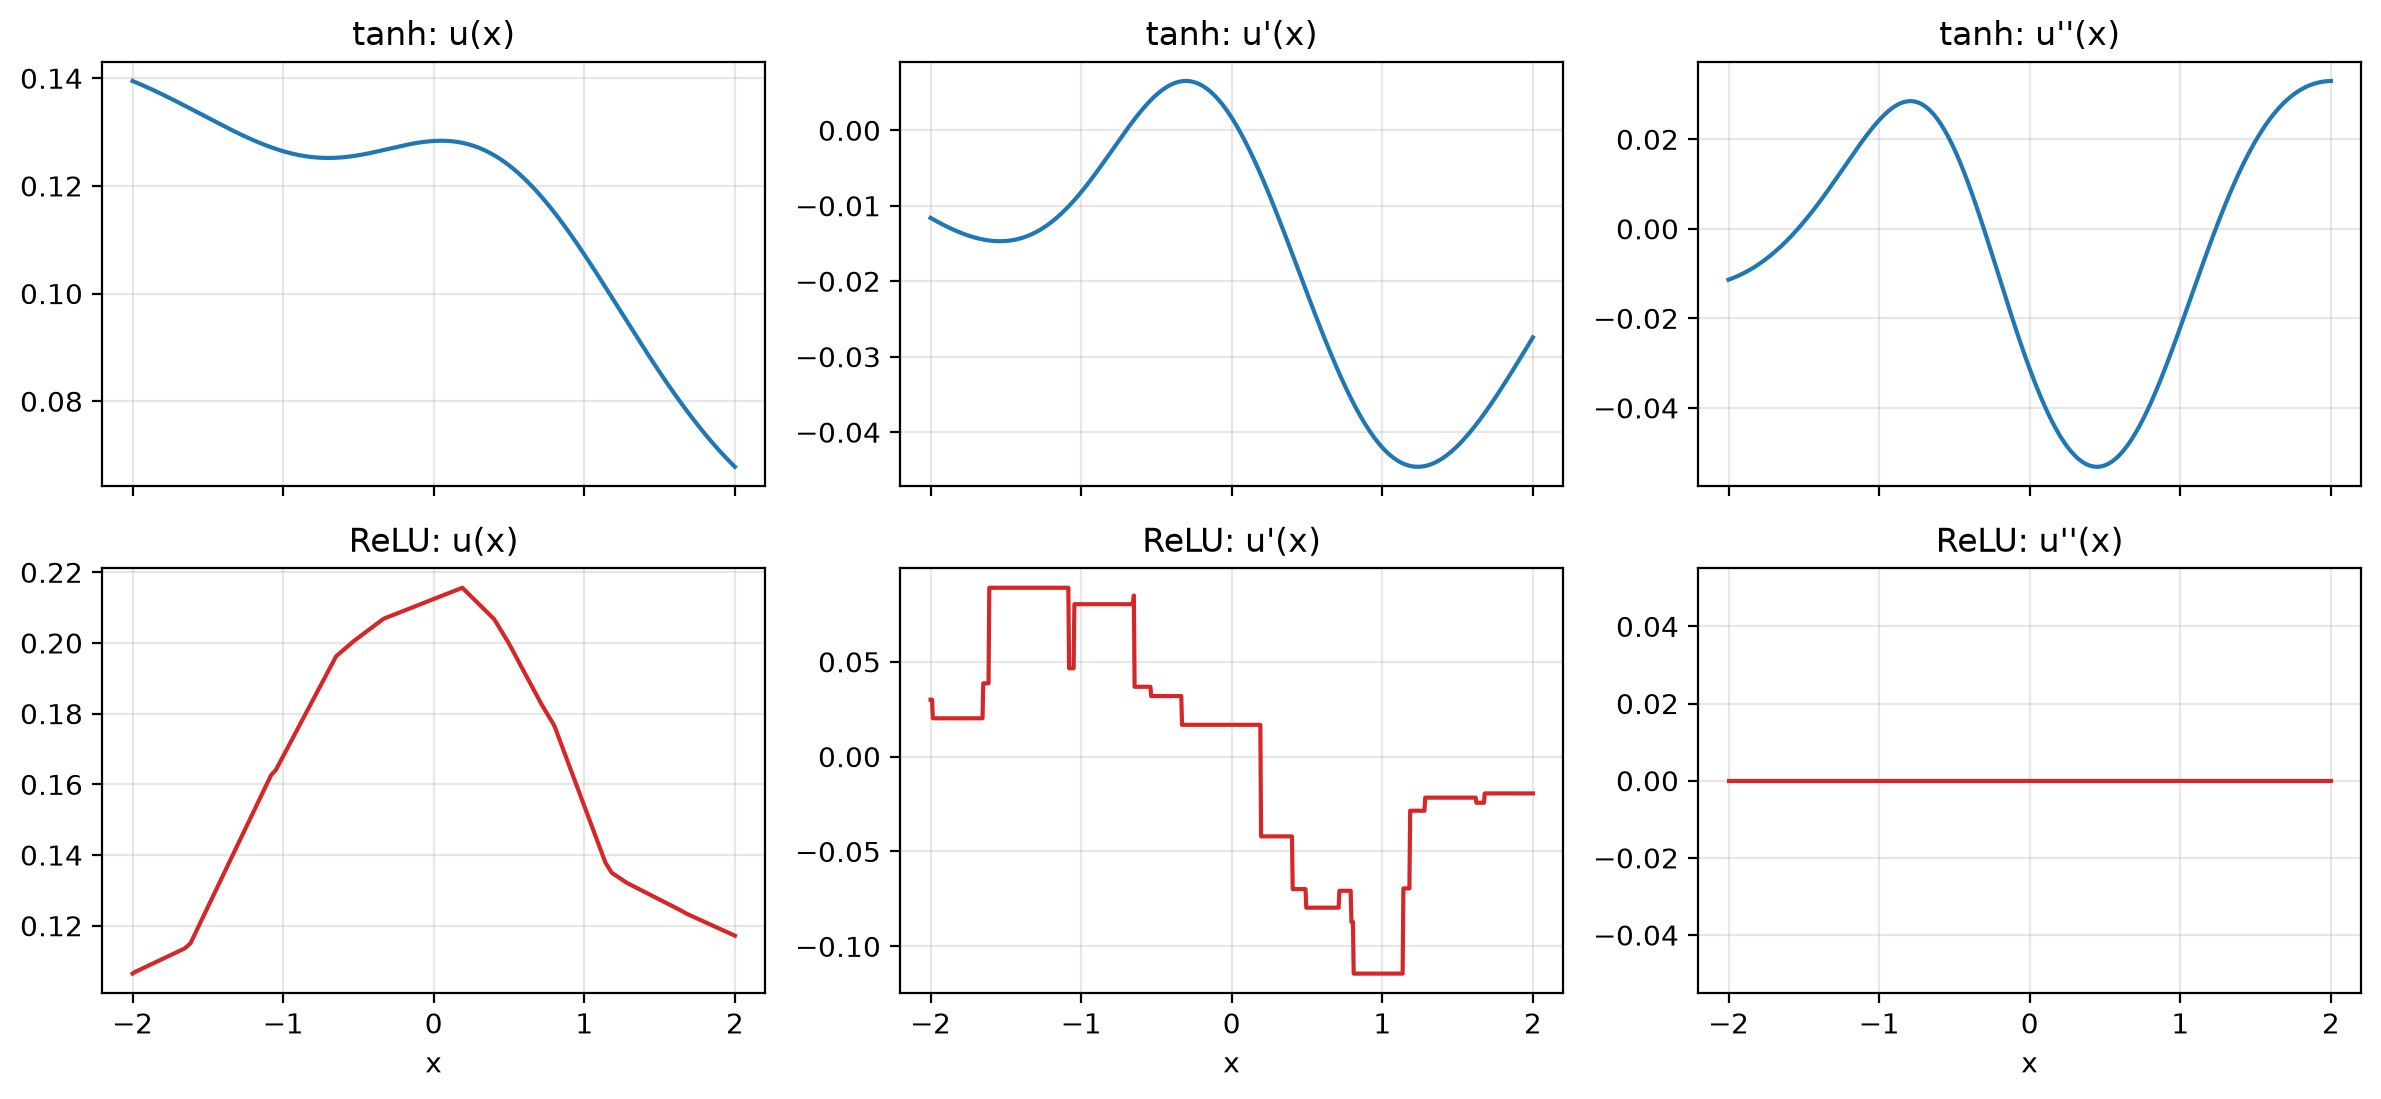
\includegraphics[width=\linewidth]{figures/tanh_vs_relu.png}
\figcap{무작위 가중치의 두 신경망 ($1\to16\to16\to1$)과 도함수 (autograd).}
\end{column}
\end{columns}
\vskip2mm
\begin{thinkbox}[ReLU로 PINN을 만들면 오류가 나는가?]
\small 나지 않는다. $u_{xx}=0$이므로 $r=-f$가 $\theta$와 무관해져 PDE 항의 gradient가 $0$이 되고, 학습은 \textbf{오류 없이 실패}한다.
PINN에는 $\tanh$, $\sin$, softplus, SiLU처럼 매끄러운 활성화 함수를 쓴다.
\end{thinkbox}
\end{frame}

% =================================================
\section{계산 그래프로 끝까지 따라가기}
% =================================================

\begin{frame}{가장 작은 신경망과 그 계산 그래프}
\[
u(x)=w_2\tanh(w_1x+b_1)+b_2,\qquad w_1=0.8,\ b_1=-0.2,\ w_2=1.5,\ b_2=0.3,\quad x=1
\]
\[
a=w_1x+b_1=0.6,\qquad h=\tanh(a)=0.53705,\qquad u=w_2h+b_2=1.10557.
\]
\centering
\begin{adjustbox}{max width=\linewidth}
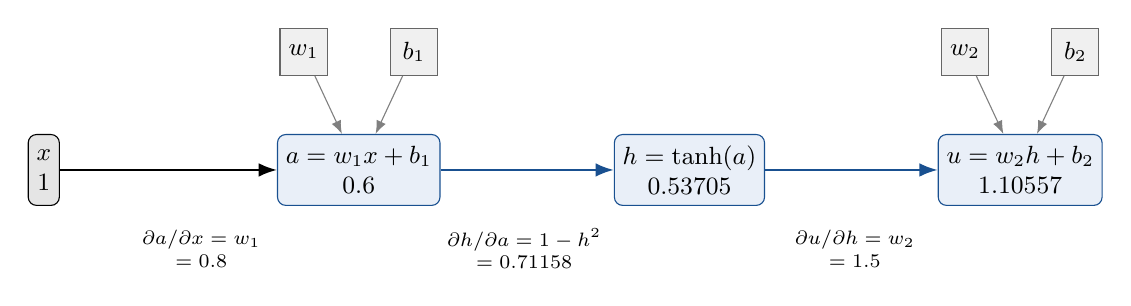
\begin{tikzpicture}
\node[val=black] (x) at (0,0) {$x$\\$1$};
\node[val=fwd] (a) at (4.0,0) {$a=w_1x+b_1$\\$0.6$};
\node[val=fwd] (h) at (8.2,0) {$h=\tanh(a)$\\$0.53705$};
\node[val=fwd] (u) at (12.4,0) {$u=w_2h+b_2$\\$1.10557$};
\node[par] (w1) at (3.3,1.5) {$w_1$}; \node[par] (b1) at (4.7,1.5) {$b_1$};
\node[par] (w2) at (11.7,1.5) {$w_2$}; \node[par] (b2) at (13.1,1.5) {$b_2$};
\draw[eg=black] (x) -- (a);
\draw[eg=fwd] (a) -- (h);
\draw[eg=fwd] (h) -- (u);
\node[font=\scriptsize,align=center] at (2.0,-1.0) {$\partial a/\partial x=w_1$\\$=0.8$};
\node[font=\scriptsize,align=center] at (6.1,-1.0) {$\partial h/\partial a=1-h^2$\\$=0.71158$};
\node[font=\scriptsize,align=center] at (10.3,-1.0) {$\partial u/\partial h=w_2$\\$=1.5$};
\foreach \p/\q in {w1/a,b1/a,w2/u,b2/u} \draw[->,black!50] (\p) -- (\q);
\end{tikzpicture}
\end{adjustbox}
\figcap{원래 계산 그래프 (forward). 둥근 상자는 중간값, 네모는 가중치 (잎 노드). 화살표 아래는 \textbf{국소 미분}.}
\figcap{숫자는 \texttt{autograd\_tiny.py}의 출력이며, 손계산과 소수점 다섯째 자리까지 일치한다.}
\end{frame}

\begin{frame}{입력에 대한 미분: 미분 그래프가 새로 생긴다}
연쇄법칙: $x$에서 $u$까지의 국소 미분을 모두 곱한다. $s=1-h^2$로 두면
\[
u_x=\pd{u}{h}\,\pd{h}{a}\,\pd{a}{x}=w_2\cdot s\cdot w_1=1.5\times0.71158\times0.8=0.85389.
\]
\centering
\begin{adjustbox}{max width=0.9\linewidth,max totalheight=4.3cm}
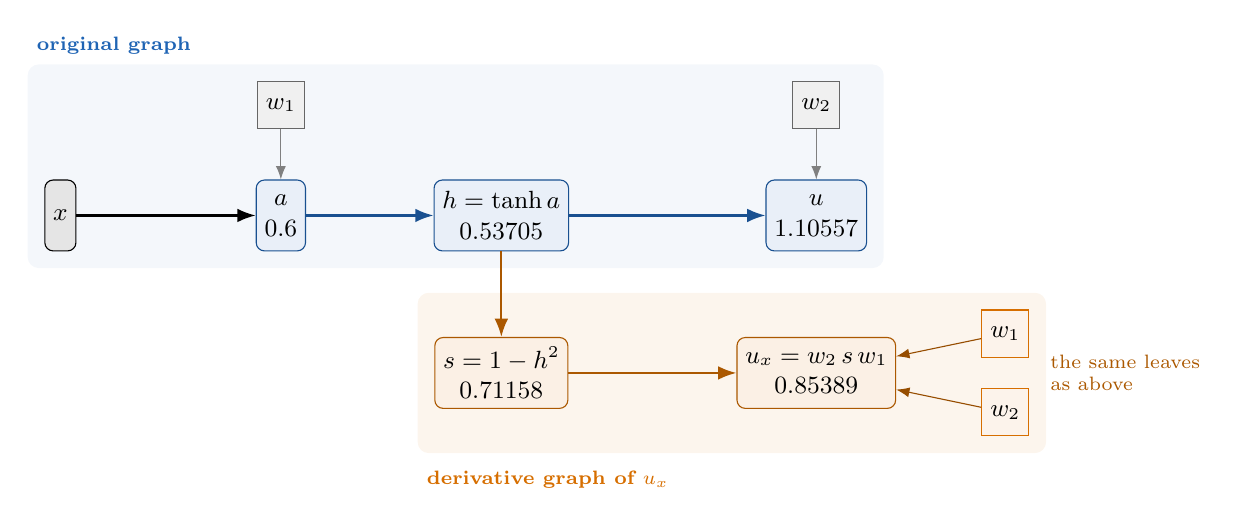
\begin{tikzpicture}
\node[val=black] (x) at (0,0) {$x$};
\node[val=fwd] (a) at (2.8,0) {$a$\\$0.6$};
\node[val=fwd] (h) at (5.6,0) {$h=\tanh a$\\$0.53705$};
\node[val=fwd] (u) at (9.6,0) {$u$\\$1.10557$};
\node[par] (w1) at (2.8,1.4) {$w_1$};
\node[par] (w2) at (9.6,1.4) {$w_2$};
\draw[eg=black] (x) -- (a); \draw[eg=fwd] (a) -- (h); \draw[eg=fwd] (h) -- (u);
\draw[->,black!50] (w1) -- (a); \draw[->,black!50] (w2) -- (u);
\node[val=der] (s) at (5.6,-2.0) {$s=1-h^2$\\$0.71158$};
\node[val=der] (ux) at (9.6,-2.0) {$u_x=w_2\,s\,w_1$\\$0.85389$};
\draw[eg=der] (h) -- (s);
\draw[eg=der] (s) -- (ux);
\node[par,draw=der,fill=der!8] (w1c) at (12.0,-1.5) {$w_1$};
\node[par,draw=der,fill=der!8] (w2c) at (12.0,-2.5) {$w_2$};
\draw[->,der!70!black] (w1c) -- (ux); \draw[->,der!70!black] (w2c) -- (ux);
\node[font=\scriptsize,der!80!black,align=left,anchor=west] at (12.45,-2.0) {the same leaves\\as above};
\begin{scope}[on background layer]
\node[fill=fwd!5,rounded corners,fit=(x)(a)(h)(u)(w1)(w2),inner sep=6pt] (F) {};
\node[fill=der!7,rounded corners,fit=(s)(ux)(w1c)(w2c),inner sep=6pt] (D) {};
\end{scope}
\node[font=\scriptsize\bfseries,fwd,anchor=south west] at (F.north west) {original graph};
\node[font=\scriptsize\bfseries,der,anchor=north west] at ([yshift=-1mm]D.south west) {derivative graph of $u_x$};
\end{tikzpicture}
\end{adjustbox}
\figcap{파란색: 원래 그래프, 주황색: $u_x$를 계산하는 미분 그래프. 미분 그래프는 원래 그래프의 $h$, $w_1$, $w_2$를 재료로 쓴다.}
\end{frame}

\begin{frame}{한 번 더 미분하기: $u_{xx}$}
\begin{keybox}[관찰 1: $u_x$는 숫자가 아니라 새로운 계산이다]
\small $u_x$를 계산하려면 원래 그래프의 $h$와 가중치 $w_1,w_2$로 새 연산을 해야 한다. 이 연산들이 \textbf{미분 그래프}를 이루며, 원래 그래프의 노드를 \textbf{공유}한다.
\end{keybox}
$u_x=w_2\,w_1\,s$에서 $w_1,w_2$는 $x$와 무관하고, $s=1-h^2$는 $a$를 통해 $x$에 의존한다.
\[
\pd{s}{a}=-2h\,\pd{h}{a}=-2hs,\qquad
u_{xx}=w_2\,w_1\,\pd{s}{a}\,\pd{a}{x}=w_2\,w_1^2\,(-2hs).
\]
숫자를 넣으면 $-2hs=-0.76431$, $\ u_{xx}=1.5\times0.64\times(-0.76431)=-0.73373$.

\vskip1mm
\begin{columns}[c,onlytextwidth]
\begin{column}{0.48\textwidth}
\small
\begin{tabular}{@{}lcccc@{}}
\toprule
텐서 & $u$ & $u_x$ & $u_{xx}$ & $\loss$ \\
\midrule
노드 수 & $10$ & $10$ & $14$ & $19$ \\
\bottomrule
\end{tabular}
\end{column}
\begin{column}{0.5\textwidth}
\small 그래프의 노드 수 (잎 포함, \texttt{autograd\_tiny.py}). 미분할 때마다 그래프가 커지므로, PINN 한 step의 계산량과 메모리는 보통 학습보다 크다.
\end{column}
\end{columns}
\end{frame}

\begin{frame}{residual과 loss: 원래 그래프와 미분 그래프가 만나는 곳}
\small 예: $u''+u=0$.\quad $x=1$에서 $r=u_{xx}+u=-0.73373+1.10557=0.37184$,\quad $\loss=r^2=0.13827$.
\vskip1mm
\centering
\begin{adjustbox}{max width=\linewidth,max totalheight=5.3cm}
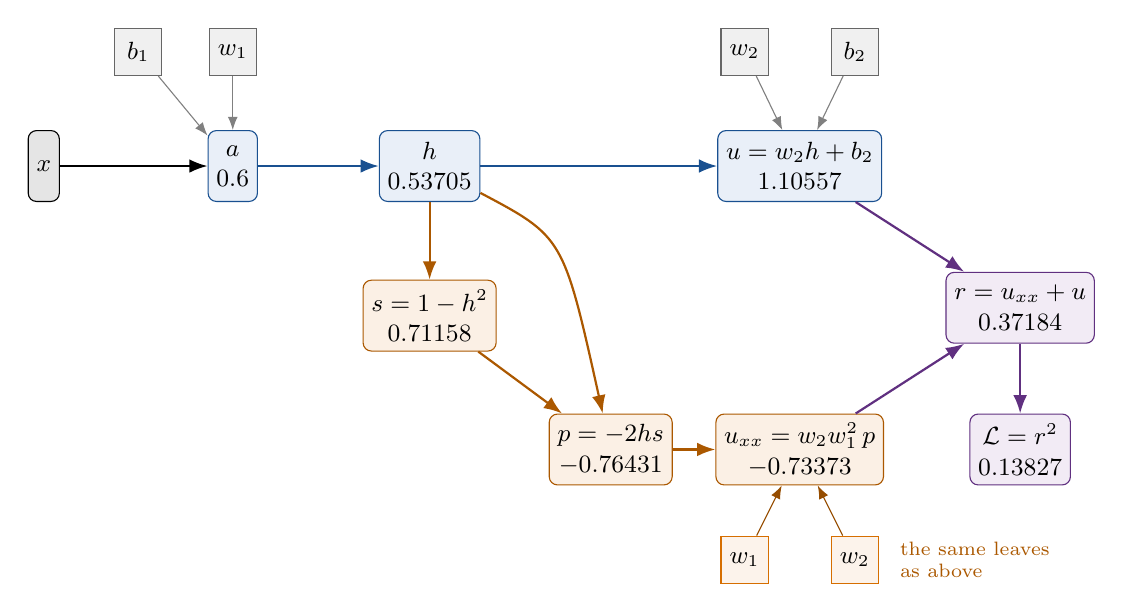
\begin{tikzpicture}
\node[val=black] (x) at (0,0) {$x$};
\node[val=fwd] (a) at (2.4,0) {$a$\\$0.6$};
\node[val=fwd] (h) at (4.9,0) {$h$\\$0.53705$};
\node[val=fwd] (u) at (9.6,0) {$u=w_2h+b_2$\\$1.10557$};
\node[par] (w1) at (2.4,1.45) {$w_1$}; \node[par] (b1) at (1.2,1.45) {$b_1$};
\node[par] (w2) at (8.9,1.45) {$w_2$}; \node[par] (b2) at (10.3,1.45) {$b_2$};
\draw[eg=black] (x) -- (a); \draw[eg=fwd] (a) -- (h); \draw[eg=fwd] (h) -- (u);
\draw[->,black!50] (w1) -- (a); \draw[->,black!50] (b1) -- (a);
\draw[->,black!50] (w2) -- (u); \draw[->,black!50] (b2) -- (u);
\node[val=der] (s) at (4.9,-1.9) {$s=1-h^2$\\$0.71158$};
\node[val=der] (p) at (7.2,-3.6) {$p=-2hs$\\$-0.76431$};
\node[val=der] (uxx) at (9.6,-3.6) {$u_{xx}=w_2w_1^2\,p$\\$-0.73373$};
\draw[eg=der] (h) -- (s);
\draw[eg=der] (s) -- (p);
\draw[eg=der] (h) .. controls (6.6,-0.9) .. (p);
\draw[eg=der] (p) -- (uxx);
\node[par,draw=der,fill=der!8] (w1c) at (8.9,-5.0) {$w_1$}; \node[par,draw=der,fill=der!8] (w2c) at (10.3,-5.0) {$w_2$};
\draw[->,der!70!black] (w1c) -- (uxx); \draw[->,der!70!black] (w2c) -- (uxx);
\node[font=\scriptsize,der!80!black,align=left,anchor=west] at (10.75,-5.0) {the same leaves\\as above};
\node[val=lossc] (r) at (12.4,-1.8) {$r=u_{xx}+u$\\$0.37184$};
\node[val=lossc] (L) at (12.4,-3.6) {$\loss=r^2$\\$0.13827$};
\draw[eg=lossc] (u) -- (r); \draw[eg=lossc] (uxx) -- (r); \draw[eg=lossc] (r) -- (L);
\end{tikzpicture}
\end{adjustbox}
\figcap{파란색: 원래 그래프, 주황색: 미분 그래프, 보라색: residual과 loss. $w_1$, $w_2$는 \textbf{양쪽에} 들어간다.}
\end{frame}

\begin{frame}{관찰 2: loss는 하나의 큰 그래프의 출력이다}
\begin{keybox}[관찰 2]
\begin{itemize}
\item residual $r$에서 원래 그래프와 미분 그래프가 \textbf{하나의 그래프}가 된다
\item PyTorch에게 미분 그래프는 특별한 것이 아니다: 덧셈, 곱셈, tanh 노드로 이루어진 그래프이고 그 끝에 스칼라 $\loss$가 있다
\item 따라서 \texttt{loss.backward()}는 보통의 역전파와 같다
\end{itemize}
\end{keybox}
\vskip3mm
\texttt{loss.backward()}는 $\loss$에서 그래프를 거꾸로 따라가며 $\partial\loss/\partial\theta$를 구한다.
한 가중치가 그래프의 여러 곳에 나타나면 \textbf{경로별 기여를 더한다} (다변수 연쇄법칙).
\vskip2mm
$\loss=r^2$이므로 $\partial\loss/\partial\theta=2r\cdot\partial r/\partial\theta$, $\ 2r=0.74368$.\quad
$r=w_2w_1^2\,p+w_2h+b_2$.
\end{frame}

\begin{frame}{역전파: gradient는 여러 경로를 거쳐 더해진다}
\small
\textbf{$b_2$}: $u$에만 있다. 경로 하나, $\partial r/\partial b_2=1$.\qquad
\textbf{$w_2$}: $u$와 $u_{xx}$ 두 곳.\ \
$\displaystyle\pd{r}{w_2}=\underbrace{h}_{\text{via }u}+\underbrace{w_1^2\,p}_{\text{via }u_{xx}}=0.53705-0.48916=0.04789$
\vskip1mm
\textbf{$w_1$}: 경로가 \textbf{세 개}.
\begin{columns}[c,onlytextwidth]
\begin{column}{0.45\textwidth}
\centering
\begin{adjustbox}{max width=\linewidth}
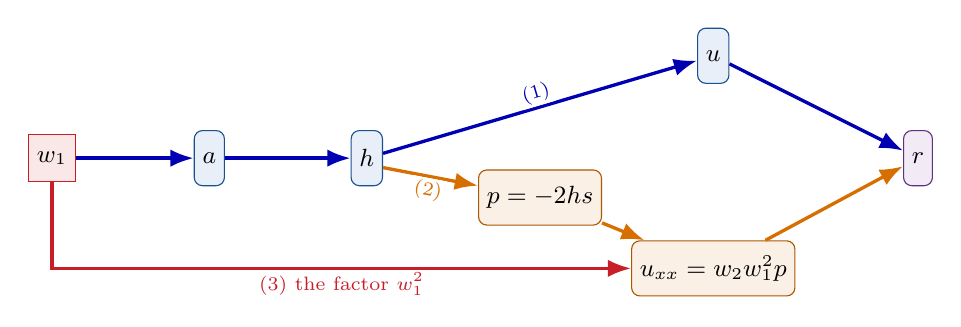
\begin{tikzpicture}
\node[par,fill=bwd!10,draw=bwd] (w1) at (0,0) {$w_1$};
\node[sval=fwd] (a) at (2.0,0) {$a$};
\node[sval=fwd] (h) at (4.0,0) {$h$};
\node[sval=fwd] (u) at (8.4,1.3) {$u$};
\node[sval=der] (p) at (6.2,-0.5) {$p=-2hs$};
\node[sval=der] (uxx) at (8.4,-1.4) {$u_{xx}=w_2w_1^2p$};
\node[sval=lossc] (r) at (11.0,0) {$r$};
\draw[->,very thick,blue!70!black] (w1) -- (a);
\draw[->,very thick,blue!70!black] (a) -- (h);
\draw[->,very thick,blue!70!black] (h) -- node[elab,above,sloped] {(1)} (u);
\draw[->,very thick,blue!70!black] (u) -- (r);
\draw[->,very thick,der] ([yshift=-1.2mm]h.east) -- node[elab,below,sloped] {(2)} (p);
\draw[->,very thick,der] (p) -- (uxx);
\draw[->,very thick,der] (uxx) -- (r);
\draw[->,very thick,bwd] (w1.south) |- node[elab,pos=0.75,below] {(3) the factor $w_1^2$} (uxx.west);
\end{tikzpicture}
\end{adjustbox}
\end{column}
\begin{column}{0.53\textwidth}
\begin{align*}
\pd{r}{w_1}
&=\underbrace{w_2\,s\,x}_{(1)}
+\underbrace{w_2\,w_1^2\,\pd{p}{a}\,x}_{(2)}
+\underbrace{w_2\cdot2w_1\cdot p}_{(3)}\\
&=1.06737-0.18408-1.83433\\
&=-0.95104
\end{align*}
{\footnotesize $\partial p/\partial a=-2s(1-3h^2)=-0.19175$}
\end{column}
\end{columns}
\vskip1mm
(1)은 보통의 역전파 경로, (2), (3)은 미분 그래프를 지나는 경로. 이 예에서는 (2)+(3)의 기여 $-2.02$가 (1)의 $1.07$보다 크고 부호가 반대이다.
\vskip1mm
\textbf{$b_1$}: $a$에서 $r$로 가는 경로 (1), (2). $\ \partial r/\partial b_1=1.06737-0.18408=0.88329$.
\end{frame}

\begin{frame}{손계산과 autograd의 비교}
\begin{center}
\begin{tabular}{@{}lcccc@{}}
\toprule
& $w_1$ & $b_1$ & $w_2$ & $b_2$ \\
\midrule
손계산 $2r\cdot\partial r/\partial\theta$ & $-0.70727$ & $0.65689$ & $0.03562$ & $0.74368$ \\
autograd (\texttt{.grad}) & $-0.70727$ & $0.65689$ & $0.03562$ & $0.74368$ \\
\bottomrule
\end{tabular}
\end{center}
\vskip3mm
\begin{thinkbox}[활성화 함수는 몇 번 미분 가능해야 하는가]
경로 (2)의 $\partial p/\partial a$는 $\tanh$의 \textbf{3계 도함수}이다. loss의 $u_{xx}$를 다시 가중치로 미분하기 때문이다.
\vskip1mm
residual에 $k$계 도함수가 있으면 역전파에는 활성화 함수의 $(k+1)$계 도함수가 필요하다.
PyTorch는 이것도 그래프로 처리한다.
\end{thinkbox}
\end{frame}

\begin{frame}{학습 한 step에서 일어나는 일}
\centering
\begin{adjustbox}{max width=\linewidth}
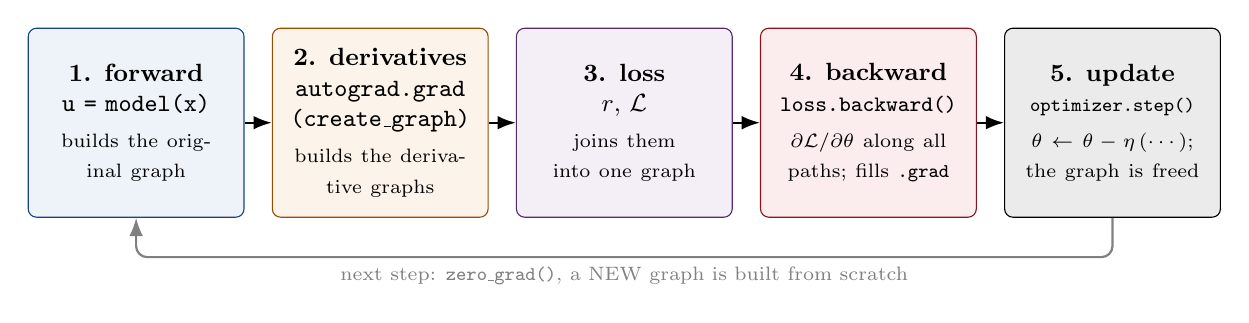
\begin{tikzpicture}
\node[st=fwd] (s1) at (0,0) {\textbf{1. forward}\\\texttt{u = model(x)}\\[2pt]{\scriptsize builds the original graph}};
\node[st=der] (s2) at (3.1,0) {\textbf{2. derivatives}\\\texttt{autograd.grad}\\\texttt{(create\_graph)}\\[2pt]{\scriptsize builds the derivative graphs}};
\node[st=lossc] (s3) at (6.2,0) {\textbf{3. loss}\\$r$, $\loss$\\[2pt]{\scriptsize joins them into one graph}};
\node[st=bwd] (s4) at (9.3,0) {\textbf{4. backward}\\{\footnotesize\texttt{loss.backward()}}\\[2pt]{\scriptsize $\partial\loss/\partial\theta$ along all paths; fills \texttt{.grad}}};
\node[st=black] (s5) at (12.4,0) {\textbf{5. update}\\{\scriptsize\texttt{optimizer.step()}}\\[2pt]{\scriptsize $\theta\leftarrow\theta-\eta\,(\cdots)$; the graph is freed}};
\foreach \i/\j in {s1/s2,s2/s3,s3/s4,s4/s5} \draw[->,thick] (\i) -- (\j);
\draw[->,thick,black!50,rounded corners] (s5.south) -- ++(0,-0.5) -| node[pos=0.25,below,font=\scriptsize] {next step: \texttt{zero\_grad()}, a NEW graph is built from scratch} (s1.south);
\end{tikzpicture}
\end{adjustbox}
\vskip2mm
\begin{itemize}
\item 1--3단계에서 그래프가 만들어진다. 2단계의 미분은 값을 계산하면서 그 계산을 그래프에 기록한다
\item 4단계는 그래프를 거꾸로 한 번 지나간다. 보통의 역전파와 다른 것은 그래프의 크기뿐
\item 5단계의 optimizer는 \texttt{.grad}만 사용하며, 2단계와 무관하다
\item 그래프는 step마다 새로 만들어지고 \texttt{backward()} 후에 해제된다
\end{itemize}
\end{frame}

\begin{frame}{PINN 학습 한 step의 세 가지 미분}
\begin{keybox}[세 가지 미분]
\begin{enumerate}
\item \texttt{torch.autograd.grad(u, x, create\_graph=True)}: \textbf{입력}에 대한 미분 $u_x$, $u_{xx}$.
결과를 돌려주고, 계산 과정을 그래프에 \textbf{추가}한다.
\vskip1mm
\item \texttt{loss.backward()}: \textbf{가중치}에 대한 미분 $\partial\loss/\partial\theta$.
원래 그래프와 미분 그래프의 모든 경로를 거쳐 더한 값을 각 가중치의 \texttt{.grad}에 넣는다.
\vskip1mm
\item \texttt{optimizer.step()}: 미분이 아니라 \textbf{갱신}. \texttt{.grad}를 이용해 가중치를 바꾼다.
\end{enumerate}
\end{keybox}
\end{frame}

% =================================================
\section{PyTorch에서 입력으로 미분하기}
% =================================================

\begin{frame}{PyTorch는 계산을 기록한다}
\centering
\begin{adjustbox}{max width=0.95\linewidth,max totalheight=2.5cm}
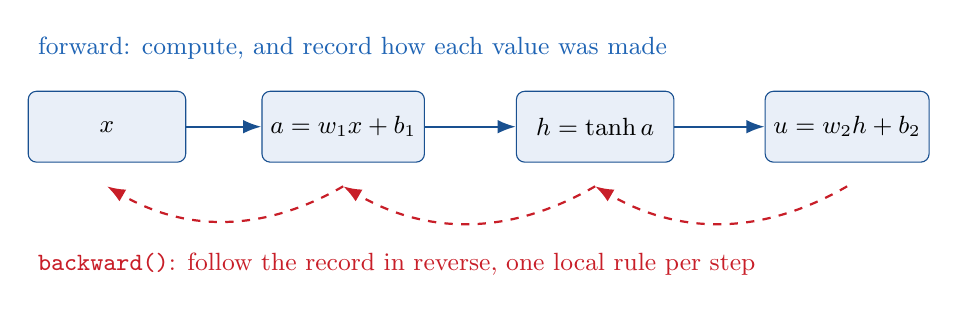
\begin{tikzpicture}
\foreach \n/\xx/\lab in {x/0/{$x$}, a/3/{$a=w_1x+b_1$}, h/6.2/{$h=\tanh a$}, u/9.4/{$u=w_2h+b_2$}}
  \node[val=fwd,minimum width=20mm] (t\n) at (\xx,0) {\lab};
\foreach \i/\j in {x/a,a/h,h/u} \draw[eg=fwd] (t\i) -- (t\j);
\foreach \i/\j in {u/h,h/a,a/x} \draw[->,thick,dashed,bwd] ([yshift=-3mm]t\i.south) to[bend left=30] ([yshift=-3mm]t\j.south);
\node[font=\small,fwd,anchor=west] at (-1,1.0) {forward: compute, and record how each value was made};
\node[font=\small,bwd,anchor=west] at (-1,-1.75) {\texttt{backward()}: follow the record in reverse, one local rule per step};
\end{tikzpicture}
\end{adjustbox}
\vskip3mm
\begin{keybox}
\begin{itemize}
\item PyTorch는 계산을 하면서 \textbf{그 과정을 기록해 둔다} (코드가 실행되는 순간에 그래프가 생긴다)
\item \texttt{backward()}는 그 기록을 \textbf{거꾸로} 따라가며 연쇄법칙을 적용한다
\item \texttt{create\_graph=True}이면 미분하는 계산 자체도 기록된다 $\Rightarrow$ 다시 미분할 수 있다
\end{itemize}
\end{keybox}
\figcap{그래프가 저장되는 방식의 세부 (\texttt{grad\_fn}, \texttt{next\_functions} 등)는 노트 4.1--4.4절과 \texttt{autograd\_tiny.py}의 8번 셀 (읽을거리).}
\end{frame}

\begin{frame}[fragile]{\texttt{x}도 추적해야 한다: \texttt{requires\_grad}}
PyTorch는 \texttt{requires\_grad=True}인 텐서에서 시작된 연산만 그래프에 기록한다.
\begin{itemize}
\item \texttt{nn.Linear}의 가중치: 기본값 \texttt{True}
\item 입력: 기본값 \texttt{False} $\Rightarrow$ $x$로 미분하려면 직접 켜야 한다
\end{itemize}
\begin{lstlisting}
x_f = torch.rand(N_f, 1)          # collocation points, shape (64, 1)
x_f.requires_grad_(True)          # now u = model(x_f) remembers how it depends on x_f
\end{lstlisting}
\vskip2mm
이때 \texttt{loss.backward()}는 \texttt{x\_f.grad}도 채우지만 (\texttt{autograd\_tiny.py}에서 \texttt{x.grad = 0.52551}) 이 값은 쓰지 않는다.
\end{frame}

\begin{frame}[fragile]{\texttt{torch.autograd.grad}와 \texttt{create\_graph}}
\small
\begin{itemize}
\item \texttt{loss.backward()}: 결과를 잎 노드의 \texttt{.grad}에 \textbf{더해 넣고}, 아무것도 돌려주지 않는다
\item \texttt{torch.autograd.grad(y, x)}: $\partial y/\partial x$를 \textbf{돌려주고} (튜플, \texttt{[0]}으로 꺼냄), \texttt{.grad}는 건드리지 않는다
\end{itemize}
\centering
\begin{adjustbox}{max width=0.92\linewidth}
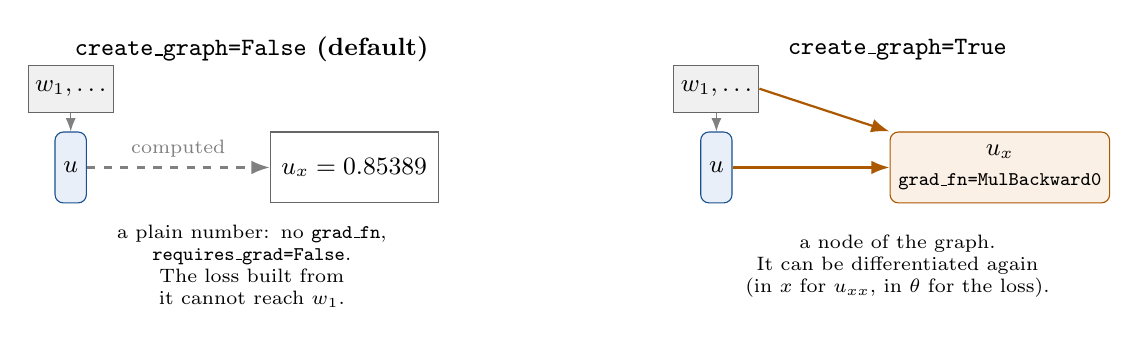
\begin{tikzpicture}
\begin{scope}
\node[font=\small\bfseries] at (2.3,1.5) {\texttt{create\_graph=False} (default)};
\node[val=fwd] (u) at (0,0) {$u$};
\node[par] (w) at (0,1.0) {$w_1,\ldots$};
\draw[->,black!50] (w) -- (u);
\node[draw=black!60,fill=white,font=\small,minimum height=9mm,inner sep=4pt] (ux) at (3.6,0) {$u_x=0.85389$};
\draw[->,thick,dashed,black!50] (u) -- node[above,font=\scriptsize] {computed} (ux);
\node[font=\scriptsize,align=center,text width=44mm] at (2.3,-1.25) {a plain number: no \texttt{grad\_fn},\\\texttt{requires\_grad=False}.\\The loss built from it cannot reach $w_1$.};
\end{scope}
\begin{scope}[xshift=8.2cm]
\node[font=\small\bfseries] at (2.3,1.5) {\texttt{create\_graph=True}};
\node[val=fwd] (u) at (0,0) {$u$};
\node[par] (w) at (0,1.0) {$w_1,\ldots$};
\draw[->,black!50] (w) -- (u);
\node[val=der] (ux) at (3.6,0) {$u_x$\\{\scriptsize \texttt{grad\_fn=MulBackward0}}};
\draw[eg=der] (u) -- (ux);
\draw[eg=der] (w.east) -- (ux.north west);
\node[font=\scriptsize,align=center,text width=44mm] at (2.3,-1.25) {a node of the graph.\\It can be differentiated again\\(in $x$ for $u_{xx}$, in $\theta$ for the loss).};
\end{scope}
\end{tikzpicture}
\end{adjustbox}
\raggedright
\vskip1mm
\texttt{create\_graph}가 없으면 $u_x$를 다시 미분할 때 오류가 난다 (\texttt{autograd\_tiny.py}의 6번 셀):
\begin{lstlisting}[language={}]
RuntimeError: element 0 of tensors does not require grad and does not have a grad_fn
\end{lstlisting}
\end{frame}

\begin{frame}[fragile]{점이 여러 개일 때: \texttt{grad\_outputs=torch.ones\_like(u)}}
\small
\texttt{x}, \texttt{u}의 모양이 $(N,1)$이면 \texttt{autograd.grad}는 \textbf{벡터--야코비 곱} $\vect v\T J$, $J_{ij}=\partial u_i/\partial x_j$를 계산한다.
샘플은 독립이므로 $u_i$는 $x_i$에만 의존한다: $J$는 \textbf{대각행렬}.
\[
\vect v=(1,\ldots,1)\ \Longrightarrow\ (\vect v\T J)_j=\sum_i \pd{u_i}{x_j}=\pd{u_j}{x_j}\quad\text{(점마다의 도함수)}
\]
\centering
\begin{adjustbox}{max width=0.85\linewidth}
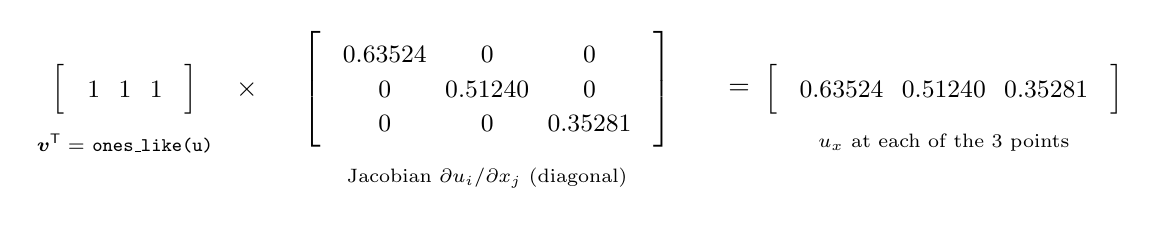
\begin{tikzpicture}
\matrix (v) [matrix of math nodes,left delimiter={[},right delimiter={]},nodes={font=\small}] at (0,0) {1 & 1 & 1\\};
\matrix (J) [matrix of math nodes,left delimiter={[},right delimiter={]},nodes={font=\small,minimum width=13mm}] at (4.6,0)
{0.63524 & 0 & 0\\ 0 & 0.51240 & 0\\ 0 & 0 & 0.35281\\};
\node at (1.55,0) {$\times$};
\node at (7.8,0) {$=$};
\matrix (r) [matrix of math nodes,left delimiter={[},right delimiter={]},nodes={font=\small}] at (10.4,0) {0.63524 & 0.51240 & 0.35281\\};
\node[font=\scriptsize,below=1mm of v] {$\vect v\T=$ \texttt{ones\_like(u)}};
\node[font=\scriptsize,below=1mm of J] {Jacobian $\partial u_i/\partial x_j$ (diagonal)};
\node[font=\scriptsize,below=1mm of r] {$u_x$ at each of the 3 points};
\end{tikzpicture}
\end{adjustbox}
\raggedright
\begin{lstlisting}
def derivative(y, x):
    return torch.autograd.grad(y, x, grad_outputs=torch.ones_like(y), create_graph=True)[0]
\end{lstlisting}
\footnotesize BatchNorm처럼 샘플을 섞는 층이 있으면 $J$가 대각이 아니어서 이 방법이 틀린다. PINN에 BatchNorm을 쓰지 않는 이유 중 하나.
\end{frame}

% =================================================
\section{첫 번째 PINN: 1차원 Poisson 방정식}
% =================================================

\begin{frame}{구조: 같은 신경망에 두 종류의 점}
\centering
\begin{adjustbox}{max width=\linewidth}
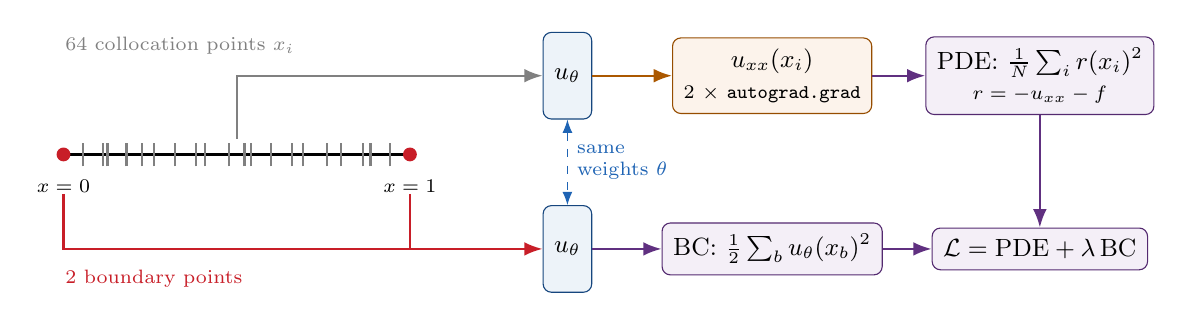
\begin{tikzpicture}
\draw[thick] (0,0) -- (4.4,0);
\foreach \t in {0.25,0.5,0.56,0.8,1.0,1.15,1.42,1.68,1.8,2.1,2.3,2.38,2.64,2.9,3.04,3.35,3.52,3.8,3.9,4.15} \draw[gray,thick] (\t,-0.15) -- (\t,0.15);
\fill[bwd] (0,0) circle (2.5pt); \fill[bwd] (4.4,0) circle (2.5pt);
\node[below,font=\scriptsize] at (0,-0.2) {$x=0$}; \node[below,font=\scriptsize] at (4.4,-0.2) {$x=1$};
\node[font=\scriptsize,gray,anchor=south west] at (-0.1,1.15) {64 collocation points $x_i$};
\node[font=\scriptsize,bwd,anchor=north west] at (-0.1,-1.35) {2 boundary points};
\node[box=fwd,minimum height=11mm] (n1) at (6.4,1.0) {$u_\theta$};
\node[box=fwd,minimum height=11mm] (n2) at (6.4,-1.2) {$u_\theta$};
\draw[<->,dashed,fwd] (n1) -- node[right,font=\scriptsize,align=left] {same\\weights $\theta$} (n2);
\draw[->,thick,gray] (2.2,0.2) |- (n1.west);
\draw[->,thick,bwd] (0,-0.5) |- (n2.west);
\draw[thick,bwd] (4.4,-0.5) -- (4.4,-1.2);
\node[box=der] (d) at (9.0,1.0) {$u_{xx}(x_i)$\\{\scriptsize 2 $\times$ \texttt{autograd.grad}}};
\node[box=lossc] (lp) at (12.4,1.0) {PDE: $\frac1N\sum_i r(x_i)^2$\\{\scriptsize $r=-u_{xx}-f$}};
\node[box=lossc] (lb) at (9.0,-1.2) {BC: $\frac12\sum_{b}u_\theta(x_b)^2$};
\node[box=lossc] (L) at (12.4,-1.2) {$\loss=\text{PDE}+\lambda\,\text{BC}$};
\draw[eg=der] (n1) -- (d); \draw[eg=lossc] (d) -- (lp);
\draw[eg=lossc] (n2) -- (lb);
\draw[eg=lossc] (lp) -- (L);
\draw[eg=lossc] (lb) -- (L);
\end{tikzpicture}
\end{adjustbox}
\figcap{collocation point에서는 미분 그래프를 거쳐 residual을, 경계에서는 값 자체를 본다.}
\end{frame}

\begin{frame}[fragile]{최소한의 코드 (1): 신경망과 점 (\texttt{pinn\_poisson\_1d\_simple.py})}
\begin{lstlisting}
torch.manual_seed(0)
device = "cuda" if torch.cuda.is_available() else "cpu"

# network u_theta: R -> R, smooth activation (tanh) so that u'' exists
model = nn.Sequential(nn.Linear(1, 32),
                      nn.Tanh(),
                      nn.Linear(32, 32),
                      nn.Tanh(),
                      nn.Linear(32, 32),
                      nn.Tanh(),
                      nn.Linear(32, 1)).to(device)

# training points: locations only, no labels
x_f = torch.rand(64, 1, device=device, requires_grad=True)     # collocation points in (0, 1): (64, 1)
x_b = torch.tensor([[0.0], [1.0]], device=device)              # boundary points: (2, 1)
\end{lstlisting}
\begin{itemize}
\item 은닉층 $3$개, 각 $32$개 뉴런, $\tanh$ (매개변수 $2209$개)
\item \texttt{requires\_grad}는 collocation point에만 켠다. 경계점에서는 미분하지 않는다
\end{itemize}
\end{frame}

\begin{frame}[fragile]{최소한의 코드 (2): 학습 루프}
\begin{lstlisting}
optimizer = torch.optim.Adam(model.parameters(), lr=1e-3)
for step in range(5000):
    u    = model(x_f)
    u_x  = torch.autograd.grad(u, x_f, grad_outputs=torch.ones_like(u),
                               create_graph=True)[0]
    u_xx = torch.autograd.grad(u_x, x_f, grad_outputs=torch.ones_like(u_x),
                               create_graph=True)[0]
    r    = -u_xx - math.pi**2 * torch.sin(math.pi * x_f)

    loss = torch.mean(r**2) + torch.mean(model(x_b)**2)   # PDE term + boundary term

    optimizer.zero_grad()
    loss.backward()        # d(loss)/d(theta), through the original and the derivative graphs
    optimizer.step()
\end{lstlisting}
\small
\begin{itemize}
\item \texttt{u}, \texttt{u\_x}, \texttt{u\_xx}: forward와 입력에 대한 미분 (1--2단계). \texttt{loss}: 3단계. \texttt{backward}, \texttt{step}: 4--5단계
\item 정확한 해 $u^*$는 학습이 끝난 뒤 $1001$개 점에서 오차를 잴 때만 쓰인다. 상대오차 $6.1\times10^{-5}$
\end{itemize}
\end{frame}

\begin{frame}{결과}
\begin{columns}[c,onlytextwidth]
\begin{column}{0.56\textwidth}
\centering
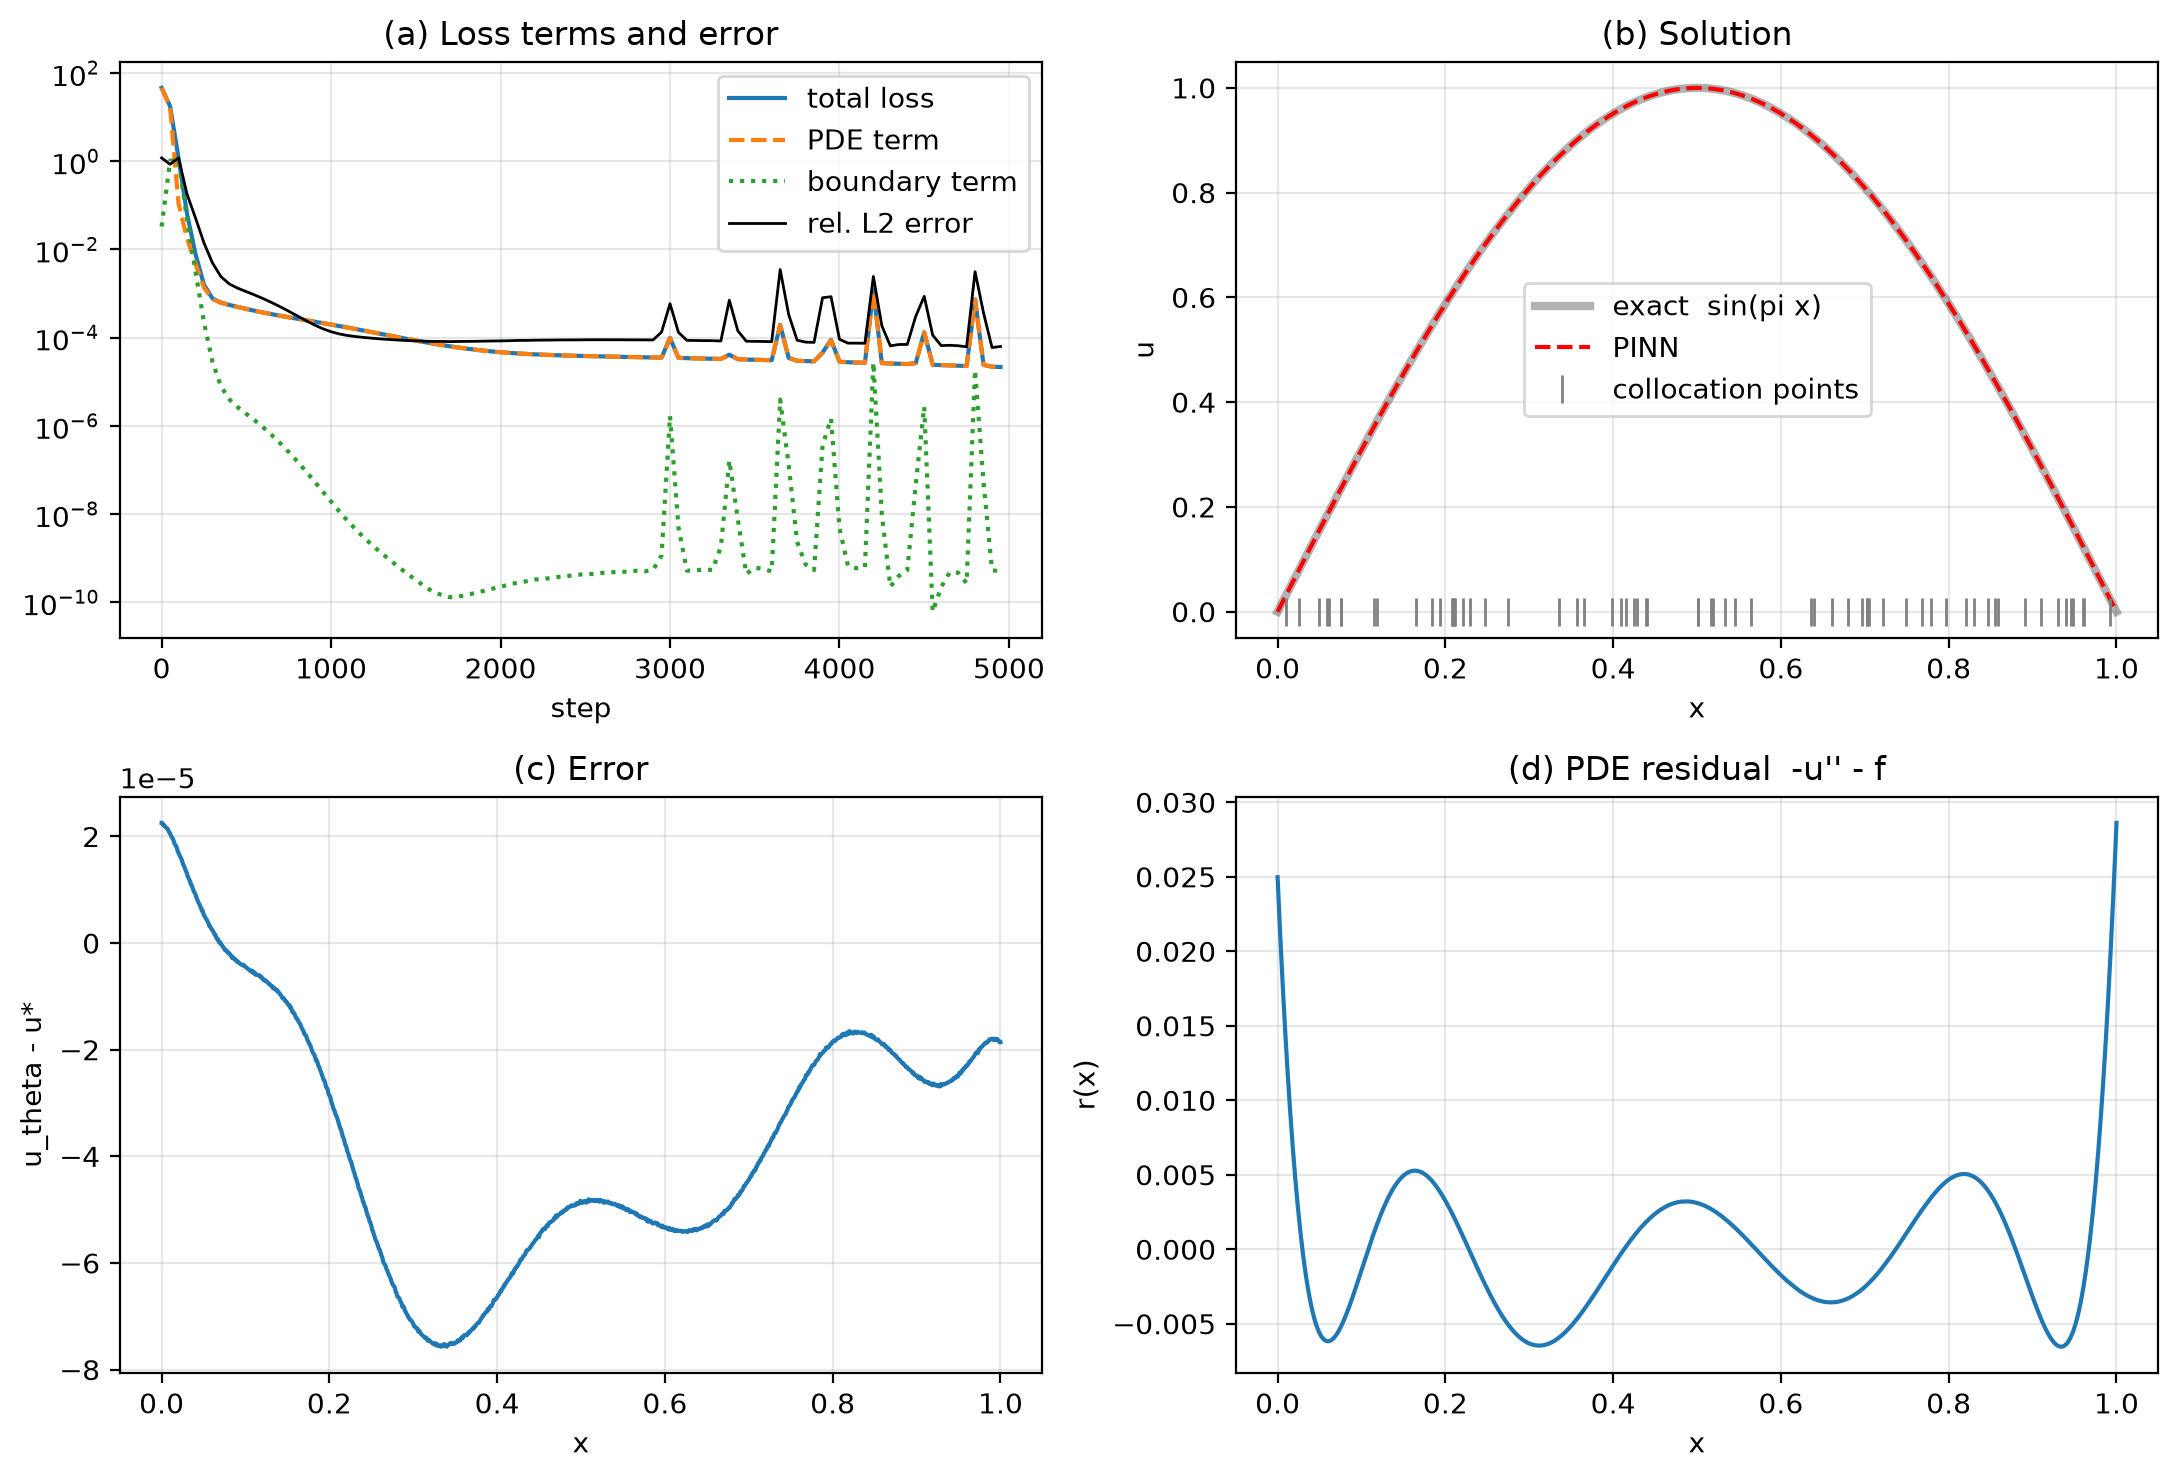
\includegraphics[width=\linewidth]{figures/poisson_result.png}
\end{column}
\begin{column}{0.42\textwidth}
\small
(a) loss와 상대오차, (b) PINN과 정확한 해, (c) 오차 $u_\theta-u^*$, (d) $[0,1]$ 전체의 residual.
\vskip1mm
\begin{itemize}
\item Adam $5000$ step, GPU (RTX 3050)에서 약 $40$초
\item 처음 loss $46.2$는 거의 PDE 항: 초기 신경망은 거의 상수 $\Rightarrow$ $r\approx-f$, $\int_0^1f^2=\pi^4/2\approx48.7$
\item 상대오차 $1000$ step $1.4\times10^{-4}$, $5000$ step $6.1\times10^{-5}$
\item $3000$ step 이후 loss가 간헐적으로 튄다 (Adam에서 흔함)
\item (d): loss에 없는 점 사이에서도 residual $\le0.03$, 양 끝 근처에서 최대
\end{itemize}
\end{column}
\end{columns}
\end{frame}

\begin{frame}{학습 중의 해: 곡률이 먼저, 경계값은 나중에}
\begin{columns}[c,onlytextwidth]
\begin{column}{0.52\textwidth}
\centering
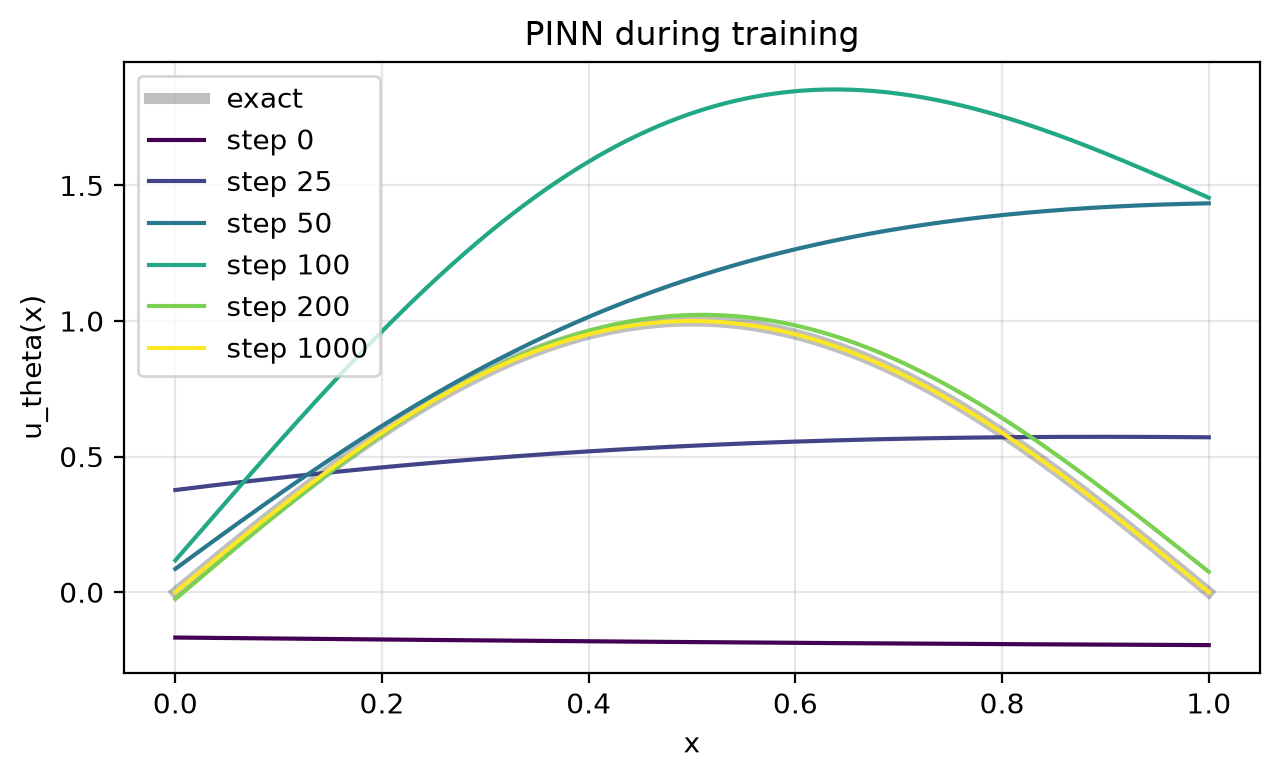
\includegraphics[width=0.92\linewidth]{figures/poisson_snapshots.png}
\end{column}
\begin{column}{0.46\textwidth}
\small
\begin{itemize}
\item $100$ step: 위로 볼록하지만 기울어져 $u(1)\approx1.45$
\item $200$ step: 양 끝이 $0$ 근처로
\item $-u''=f$의 일반해 $=$ 특수해 $+\,c_0+c_1x$. PDE 항은 $c_0$, $c_1$을 정하지 못하고, \textbf{경계 항}이 정한다
\item 초기에는 PDE 항이 훨씬 크므로 곡률이 먼저 맞는다
\end{itemize}
\end{column}
\end{columns}
\vskip2mm
\begin{remarkbox}[L-BFGS로 마무리하기]
\small Adam 뒤에 준-Newton 방법인 \textbf{L-BFGS}로 이어서 학습하면 $1$초 이내에 loss $2.1\times10^{-6}$, 상대오차 $1.5\times10^{-5}$.
미니배치가 없어 loss가 결정적인 PINN에 적합하다. 한 step에 loss를 여러 번 계산하므로 \texttt{closure}를 넘긴다.
\end{remarkbox}
\end{frame}

\begin{frame}{중간 정리}
\begin{keybox}[중간 정리]
\begin{itemize}
\item PINN은 신경망 $u_\theta$를 해의 후보로 두고, 방정식의 residual과 경계조건의 오차를 loss로 최소화한다. 정답 데이터가 필요 없다
\item $u_x$, $u_{xx}$는 \texttt{torch.autograd.grad(..., create\_graph=True)}로 구한다. 이 계산은 원래 그래프의 노드를 재료로 쓰는 \textbf{미분 그래프}를 만든다
\item residual이 원래 그래프와 미분 그래프를 하나로 잇고, \texttt{loss.backward()}는 그 전체를 거꾸로 지나간다. 한 가중치가 여러 곳에 있으면 경로마다의 기여가 \textbf{더해진다}
\item 활성화 함수는 매끄러워야 한다 ($\tanh$). ReLU는 $u''=0$이 되어 조용히 실패한다
\item \texttt{grad\_outputs=ones\_like(u)}: 야코비가 대각이므로 점마다의 도함수를 준다
\end{itemize}
\end{keybox}
\end{frame}

% =================================================
\section{시간이 있는 문제: 열 방정식}
% =================================================

\begin{frame}{열 방정식}
길이 $1$인 막대의 온도 $u(x,t)$:
\[
u_t=\kappa\,u_{xx}\quad(0<x<1,\ 0<t<1),\qquad u(x,0)=\sin(\pi x),\qquad u(0,t)=u(1,t)=0,
\]
$\kappa=0.1$ (열확산계수). $u=X(x)T(t)$를 대입하면 정확한 해는
\[
u^*(x,t)=e^{-\kappa\pi^2t}\sin(\pi x)\qquad\text{(모양은 그대로, $t=1$에서 진폭 $\approx0.37$배)}.
\]
\vskip2mm
\begin{keybox}[Poisson 문제와 다른 점]
\begin{enumerate}
\item 신경망의 입력이 $(x,t)$ \textbf{두 개}: $u_\theta:\R^2\to\R$
\item 조건이 세 종류: 방정식 (내부), \textbf{초기조건} ($t=0$), 경계조건 ($x=0,1$) $\Rightarrow$ loss의 항도 세 개
\end{enumerate}
\end{keybox}
\end{frame}

\begin{frame}{입력이 두 개일 때의 미분}
\small 입력을 \texttt{X} $(N,2)$에 모은다 (열: $x$, $t$). \texttt{grad(u, X)}는 \texttt{X}와 같은 모양 $(N,2)$이고, 각 행은 $(u_x,u_t)$.
\vskip1mm
\centering
\begin{adjustbox}{max width=\linewidth,max totalheight=4.8cm}
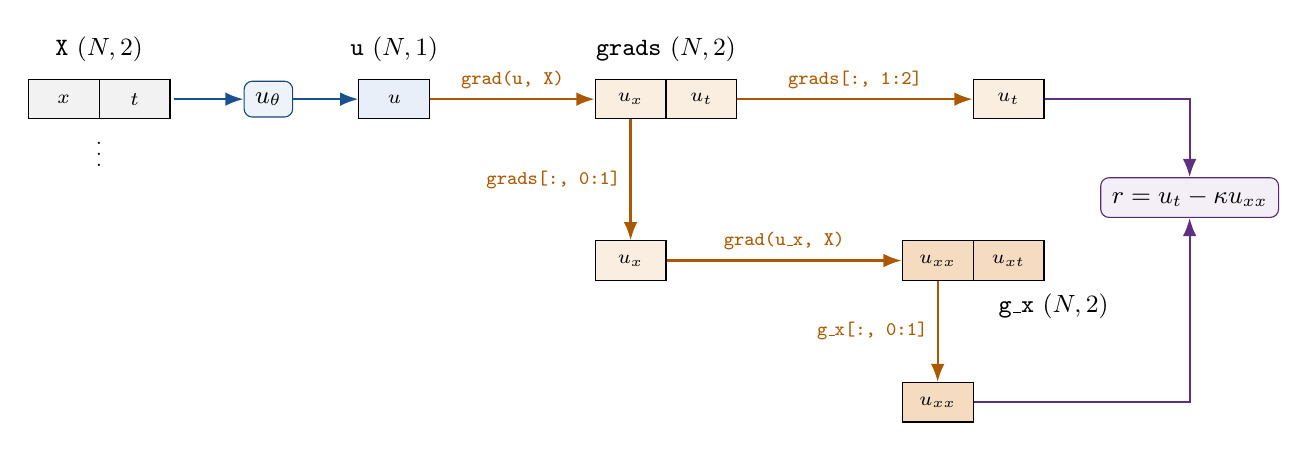
\begin{tikzpicture}[mat/.style={draw,minimum width=9mm,minimum height=5mm,font=\scriptsize,inner sep=1pt}]
\node[mat,fill=black!5] (X1) at (0,0.25) {$x$}; \node[mat,fill=black!5] (X2) at (0.9,0.25) {$t$};
\node[font=\scriptsize] at (0.45,-0.35) {$\vdots$};
\node[font=\small,above] at (0.45,0.6) {\texttt{X} $(N,2)$};
\node[box=fwd] (n) at (2.6,0.25) {$u_\theta$};
\draw[eg=fwd] (1.4,0.25) -- (n);
\node[mat,fill=fwd!10] (u) at (4.2,0.25) {$u$};
\node[font=\small,above] at (4.2,0.6) {\texttt{u} $(N,1)$};
\draw[eg=fwd] (n) -- (u);
\node[mat,fill=der!12] (g1) at (7.2,0.25) {$u_x$}; \node[mat,fill=der!12] (g2) at (8.1,0.25) {$u_t$};
\node[font=\small,above] at (7.65,0.6) {\texttt{grads} $(N,2)$};
\draw[eg=der] (u) -- node[above,font=\scriptsize] {\texttt{grad(u, X)}} (g1);
\node[mat,fill=der!12] (ux) at (7.2,-1.8) {$u_x$};
\node[mat,fill=der!12] (ut) at (12.0,0.25) {$u_t$};
\draw[eg=der] (g1.south) -- node[left,font=\scriptsize] {\texttt{grads[:, 0:1]}} (ux.north);
\draw[eg=der] (g2.east) -- node[above,font=\scriptsize] {\texttt{grads[:, 1:2]}} (ut.west);
\node[mat,fill=der!25] (h1) at (11.1,-1.8) {$u_{xx}$}; \node[mat,fill=der!25] (h2) at (12.0,-1.8) {$u_{xt}$};
\node[font=\small,anchor=north west] at (11.75,-2.1) {\texttt{g\_x} $(N,2)$};
\draw[eg=der] (ux.east) -- node[above,font=\scriptsize] {\texttt{grad(u\_x, X)}} (h1.west);
\node[mat,fill=der!25] (uxx) at (11.1,-3.6) {$u_{xx}$};
\draw[eg=der] (h1.south) -- node[left,font=\scriptsize] {\texttt{g\_x[:, 0:1]}} (uxx.north);
\node[box=lossc] (r) at (14.3,-1.0) {$r=u_t-\kappa u_{xx}$};
\draw[eg=lossc] (ut.east) -| (r.north);
\draw[eg=lossc] (uxx.east) -| (r.south);
\end{tikzpicture}
\end{adjustbox}
\figcap{필요한 열을 잘라 쓴다. $u_{xt}$도 함께 계산되지만 쓰지 않는다.}
\end{frame}

\begin{frame}[fragile]{residual 코드: 모양 $(N,1)$을 유지하자}
\begin{lstlisting}
def residual(model, X):
    u = model(X)                                     # (N, 1)
    # derivative with respect to both inputs: (N, 2), the columns are [u_x, u_t]
    grads = torch.autograd.grad(u, X, torch.ones_like(u), create_graph=True)[0]
    u_x, u_t = grads[:, 0:1], grads[:, 1:2]          # (N, 1) each
    # differentiate u_x again: (N, 2) = [u_xx, u_xt]; keep the first column
    g_x = torch.autograd.grad(u_x, X, torch.ones_like(u_x), create_graph=True)[0]
    u_xx = g_x[:, 0:1]
    return u_t - kappa * u_xx
\end{lstlisting}
\vskip2mm
\begin{thinkbox}[\texttt{grads[:, 0]}이 아니라 \texttt{grads[:, 0:1]}인 이유]
\texttt{grads[:, 0]}의 모양은 $(N,)$이다. $(N,)$과 $(N,1)$을 빼면 broadcasting 때문에 $(N,N)$ 행렬이 되어 버린다.
\texttt{u\_t}와 \texttt{u\_xx}를 모두 $(N,1)$로 유지해야 한다.
\end{thinkbox}
\end{frame}

\begin{frame}[fragile]{세 종류의 점과 세 개의 loss 항}
\[
\loss=\underbrace{\frac1{N_f}\sum_i r_i^2}_{\text{PDE}}
+\underbrace{\frac1{N_0}\sum_j\big(u_\theta(x_j,0)-\sin\pi x_j\big)^2}_{\text{initial}}
+\underbrace{\frac1{N_b}\sum_k u_\theta(x_k,t_k)^2}_{\text{boundary}}
\]
\begin{columns}[c,onlytextwidth]
\begin{column}{0.32\textwidth}
\centering
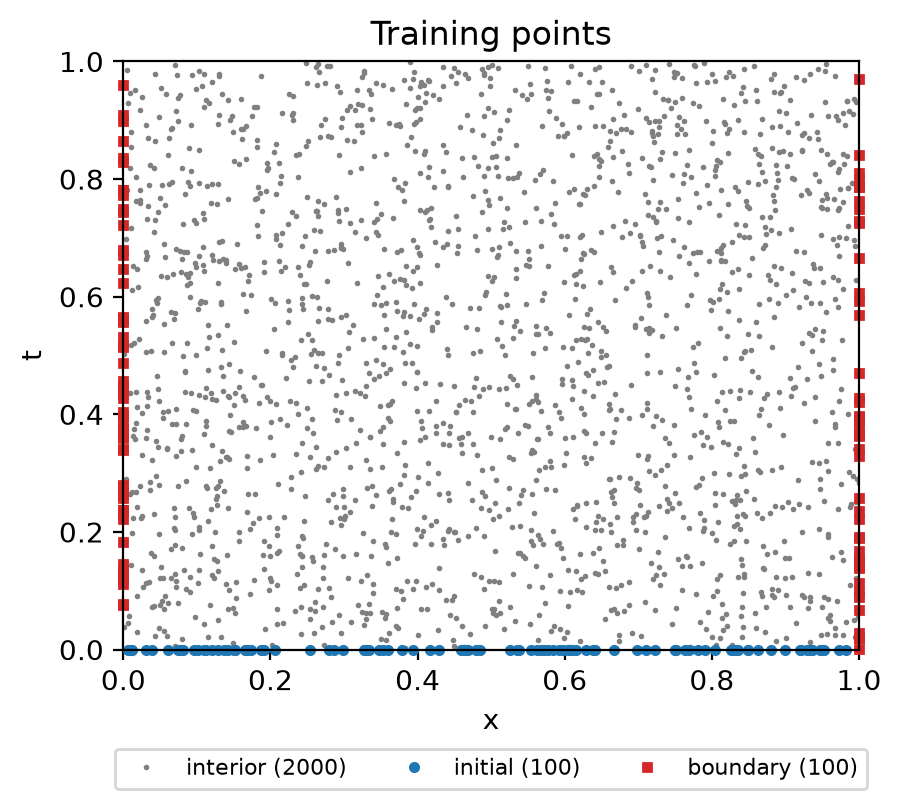
\includegraphics[width=0.8\linewidth]{figures/heat_points.png}
\figcap{내부 $N_f=2000$, 초기선 $N_0=100$, 경계선 $N_b=100$ (무작위).}
\end{column}
\begin{column}{0.66\textwidth}
\small
\begin{lstlisting}
def loss_terms(model):
    loss_pde = torch.mean(residual(model, X_f)**2)
    loss_ic  = torch.mean((model(X_0) - u_0)**2)
    loss_bc  = torch.mean((model(X_b) - u_b)**2)
    return loss_pde, loss_ic, loss_bc
\end{lstlisting}
\begin{itemize}
\item 세 항의 가중치는 모두 $1$
\item PDE 항만 미분 그래프를 거친다. 역전파는 세 항의 gradient를 각 가중치에서 더한다
\end{itemize}
\end{column}
\end{columns}
\end{frame}

\begin{frame}{결과}
\small 신경망 $2\to32\to32\to32\to1$ ($\tanh$, $2241$개), Adam $5000$ step, GPU (RTX 3050)에서 약 $2$분.
$101\times101$ 격자에서 상대오차 $1.7\times10^{-3}$, 최대 절대오차 $6.5\times10^{-3}$.
\vskip1mm
\centering
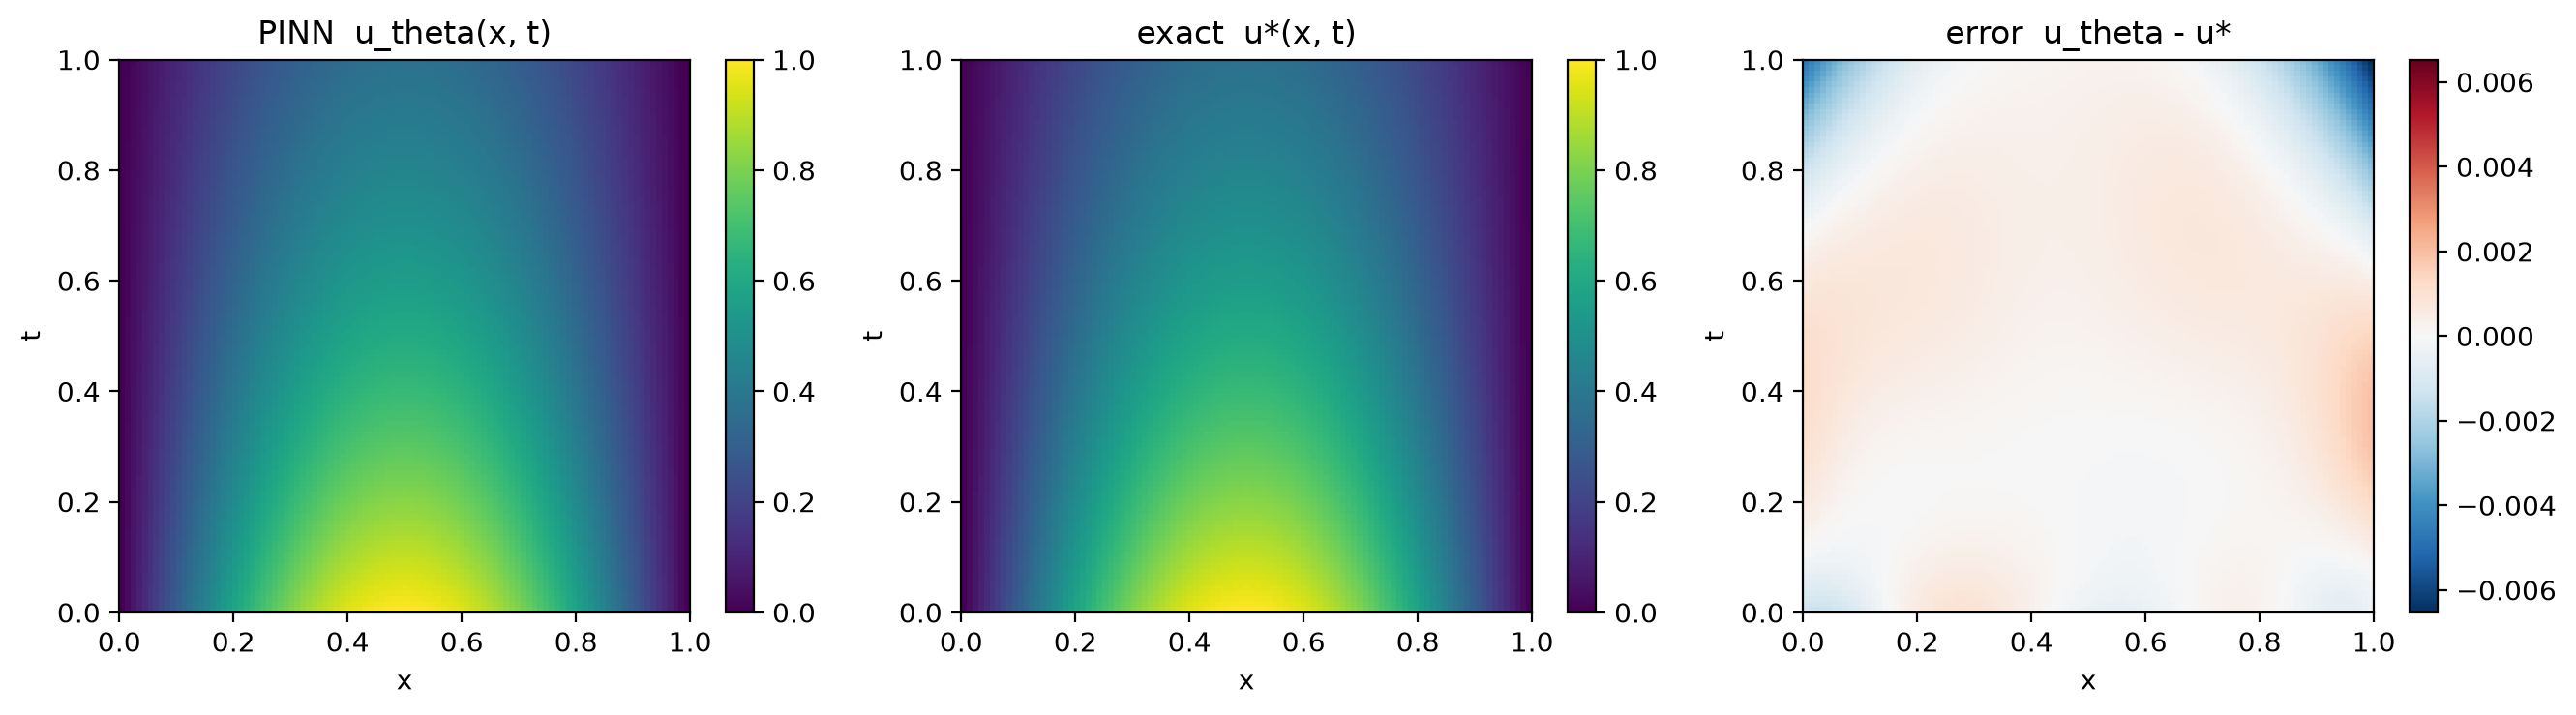
\includegraphics[width=0.9\linewidth]{figures/heat_field.png}
\figcap{왼쪽부터 PINN의 해, 정확한 해, 오차. 가로축 $x$, 세로축 시간 $t$.}
\end{frame}

\begin{frame}{학습 과정}
\centering
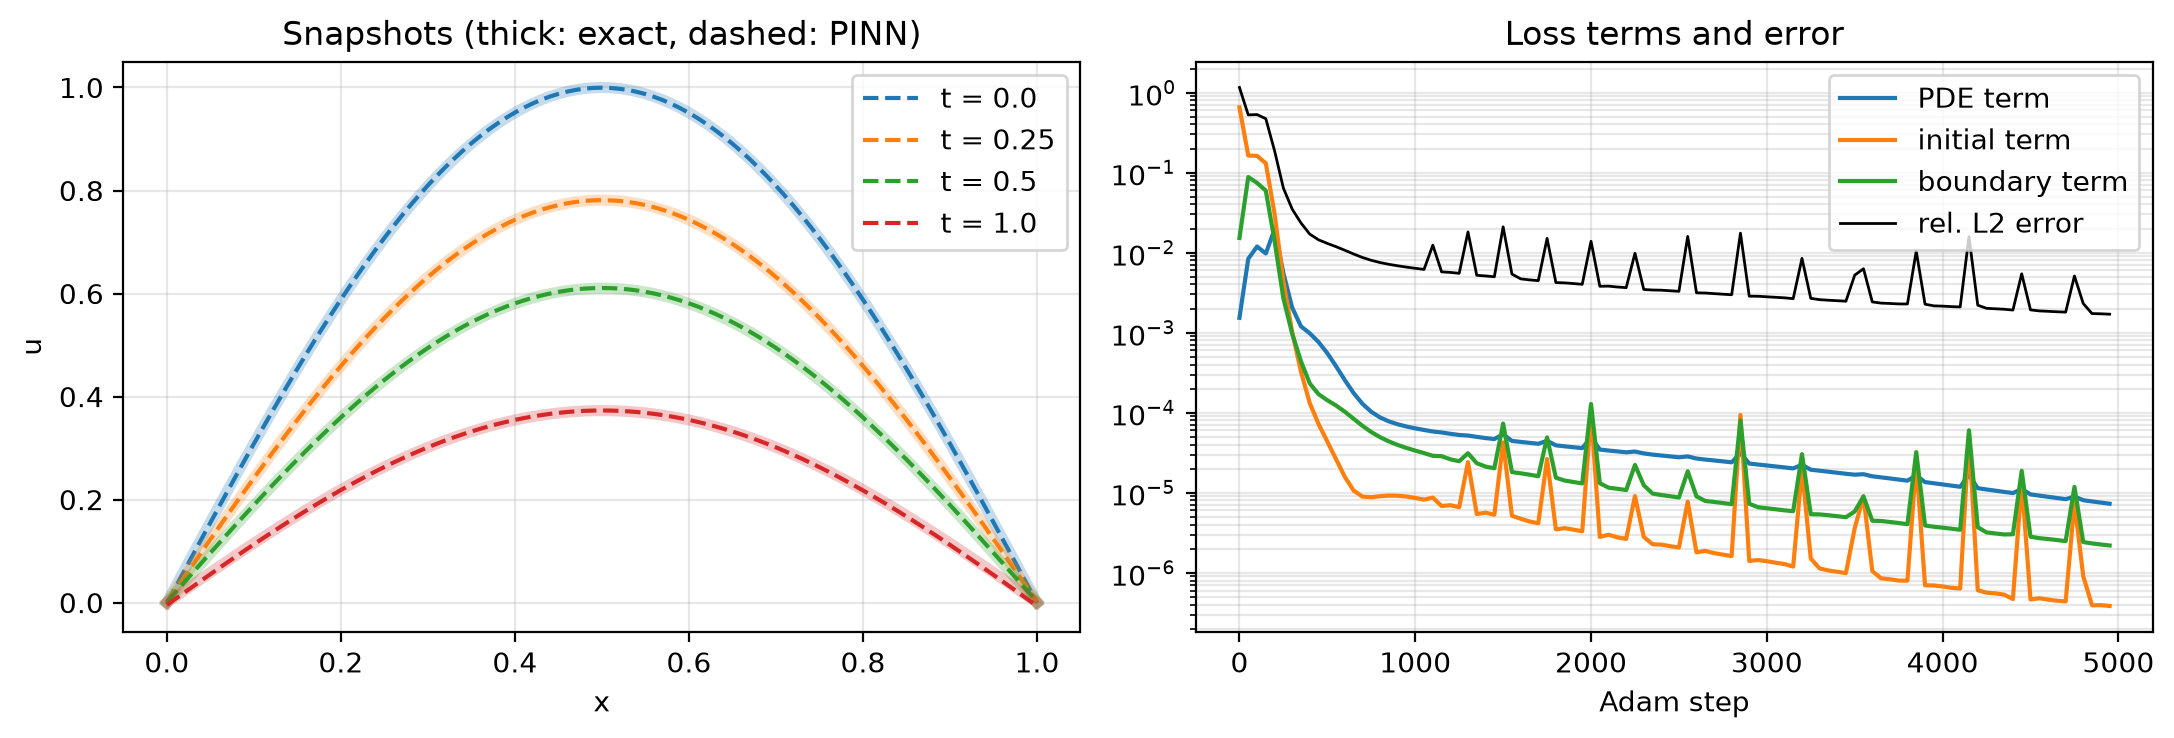
\includegraphics[width=0.9\linewidth]{figures/heat_snapshots.png}
\figcap{왼쪽: 네 시각의 단면 (굵은 선: 정확한 해, 점선: PINN). 오른쪽: loss의 세 항과 상대오차.}
\raggedright
\small
\begin{itemize}
\item 처음에 PDE 항 $1.5\times10^{-3}$, 초기조건 항 $0.65$. \textbf{상수 함수는 열 방정식의 해이다} ($u_t=0=\kappa u_{xx}$).
PDE만으로는 해가 유일하지 않고, 초기조건과 경계조건이 해를 하나로 정한다
\item 오차는 $t=1$ 근처의 두 모서리 ($x\approx0$, $x\approx1$)에서 가장 크다
\end{itemize}
\end{frame}

% =================================================
\section{역문제: 측정값에서 계수 찾기}
% =================================================

\begin{frame}{순문제와 역문제}
\centering
\begin{adjustbox}{max width=0.92\linewidth}
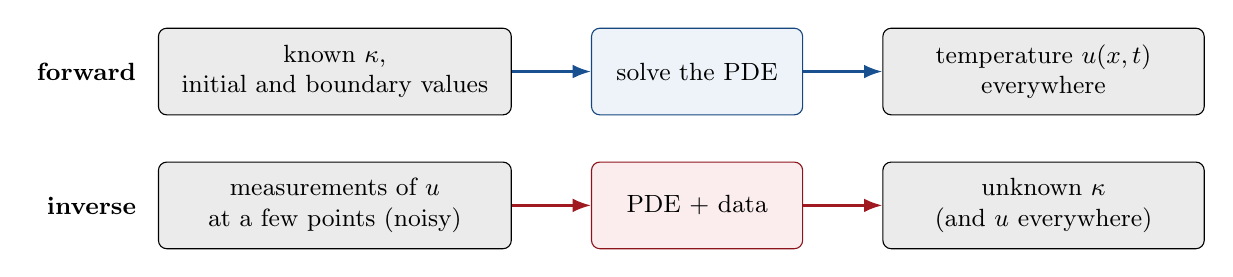
\begin{tikzpicture}
\node[box=black,text width=42mm,minimum height=11mm] (k1) at (0,0) {known $\kappa$,\\initial and boundary values};
\node[box=fwd,text width=24mm,minimum height=11mm] (s1) at (4.6,0) {solve the PDE};
\node[box=black,text width=38mm,minimum height=11mm] (u1) at (9.0,0) {temperature $u(x,t)$\\everywhere};
\draw[eg=fwd] (k1) -- (s1); \draw[eg=fwd] (s1) -- (u1);
\node[font=\small\bfseries,anchor=east] at (-2.4,0) {forward};
\node[box=black,text width=42mm,minimum height=11mm] (u2) at (0,-1.7) {measurements of $u$\\at a few points (noisy)};
\node[box=bwd,text width=24mm,minimum height=11mm] (s2) at (4.6,-1.7) {PDE + data};
\node[box=black,text width=38mm,minimum height=11mm] (k2) at (9.0,-1.7) {unknown $\kappa$\\(and $u$ everywhere)};
\draw[eg=bwd] (u2) -- (s2); \draw[eg=bwd] (s2) -- (k2);
\node[font=\small\bfseries,anchor=east] at (-2.4,-1.7) {inverse};
\end{tikzpicture}
\end{adjustbox}
\raggedright
\vskip3mm
\begin{itemize}
\item \textbf{순문제} (forward problem): 방정식, 계수, 초기·경계조건 $\to$ 해 $u$
\item \textbf{역문제} (inverse problem): $u$의 측정값 $\to$ 계수 $\kappa$
\item 예: CT, 전기 임피던스 단층촬영 (EIT), 지하 탐사, 비파괴 검사
\item 고전적으로는 $\kappa$를 바꾸어 가며 순문제를 반복해서 푼다.
PINN에서는 \textbf{$\kappa$를 신경망의 매개변수와 함께 학습}시킨다
\end{itemize}
\end{frame}

\begin{frame}[fragile]{$\kappa$를 학습 가능한 매개변수로}
\begin{lstlisting}
kappa = nn.Parameter(torch.tensor(kappa_init, device=device))   # trainable, like a weight
optimizer = torch.optim.Adam(list(model.parameters()) + [kappa], lr=1e-3)
\end{lstlisting}
\small 초깃값 $0.5$ (참값 $0.1$의 다섯 배). \texttt{nn.Parameter}는 \texttt{requires\_grad=True}인 텐서이고, optimizer에 넘기면 가중치와 같이 갱신된다.
초기·경계조건은 모른다고 가정하여 쓰지 않는다.
\[
\loss(\theta,\kappa)=\underbrace{\frac1{N_d}\sum_{j}\big(u_\theta(x_j,t_j)-u^{\text{obs}}_j\big)^2}_{\text{data}}
+\underbrace{\frac1{N_f}\sum_i\big(u_t-\kappa\,u_{xx}\big)^2\Big|_{(x_i,t_i)}}_{\text{PDE}}
\]
\centering
\begin{adjustbox}{max width=0.7\linewidth,max totalheight=2.4cm}
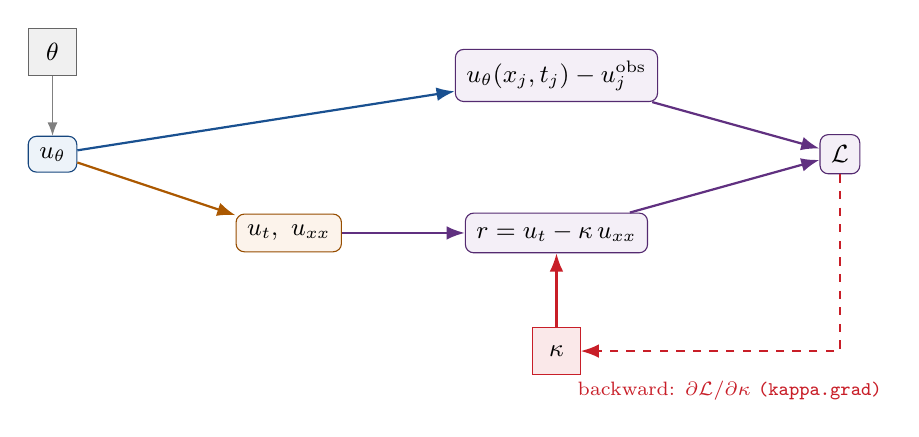
\begin{tikzpicture}
\node[box=fwd] (net) at (0,0) {$u_\theta$};
\node[box=der] (d) at (3.0,-1.0) {$u_t,\ u_{xx}$};
\node[box=lossc] (r) at (6.4,-1.0) {$r=u_t-\kappa\,u_{xx}$};
\node[box=lossc] (dat) at (6.4,1.0) {$u_\theta(x_j,t_j)-u^{\text{obs}}_j$};
\node[box=lossc] (L) at (10.0,0) {$\loss$};
\node[par,fill=bwd!10,draw=bwd] (k) at (6.4,-2.5) {$\kappa$};
\node[par] (th) at (0,1.3) {$\theta$};
\draw[->,black!50] (th) -- (net);
\draw[eg=der] (net) -- (d); \draw[eg=lossc] (d) -- (r); \draw[eg=fwd] (net) -- (dat);
\draw[->,thick,bwd] (k) -- (r);
\draw[eg=lossc] (r) -- (L); \draw[eg=lossc] (dat) -- (L);
\draw[->,dashed,thick,bwd] (L.south) |- (k.east);
\node[font=\scriptsize,bwd,anchor=north] at (8.6,-2.75) {backward: $\partial\loss/\partial\kappa$ \texttt{(kappa.grad)}};
\end{tikzpicture}
\end{adjustbox}
\end{frame}

\begin{frame}{$\kappa$의 gradient}
$\kappa$는 residual에만 들어가는 잎 노드이다. 역전파가 \texttt{kappa.grad}를 채우는 경로는 하나뿐이다.
\[
\pd{\loss}{\kappa}=\frac{2}{N_f}\sum_i r_i\,\pd{r_i}{\kappa}=\frac{2}{N_f}\sum_i r_i\,(-u_{xx,i}).
\]
\begin{itemize}
\item 측정값 항은 $u_\theta$를 측정값에 맞추고, PDE 항은 그 $u_\theta$가 만족하는 열 방정식의 $\kappa$를 정한다
\item $u_\theta$를 고정하면 PDE 항은 $\kappa$의 이차함수이고, $\partial\loss/\partial\kappa=0$에서
\[
\kappa=\frac{\sum_i u_{t,i}\,u_{xx,i}}{\sum_i u_{xx,i}^2},
\]
즉 $u_t$를 $u_{xx}$에 최소제곱으로 회귀한 기울기이다
\end{itemize}
\end{frame}

\begin{frame}{결과}
\small 측정값 $N_d=200$개 ($u^*$에 잡음 $\mathcal N(0,\sigma^2)$, $\sigma=0.05$는 약 $5\%$), collocation point $N_f=2000$개, Adam $5000$ step, 한 번에 약 $2.5$--$3$분 (RTX 3050).
\vskip1mm
\centering
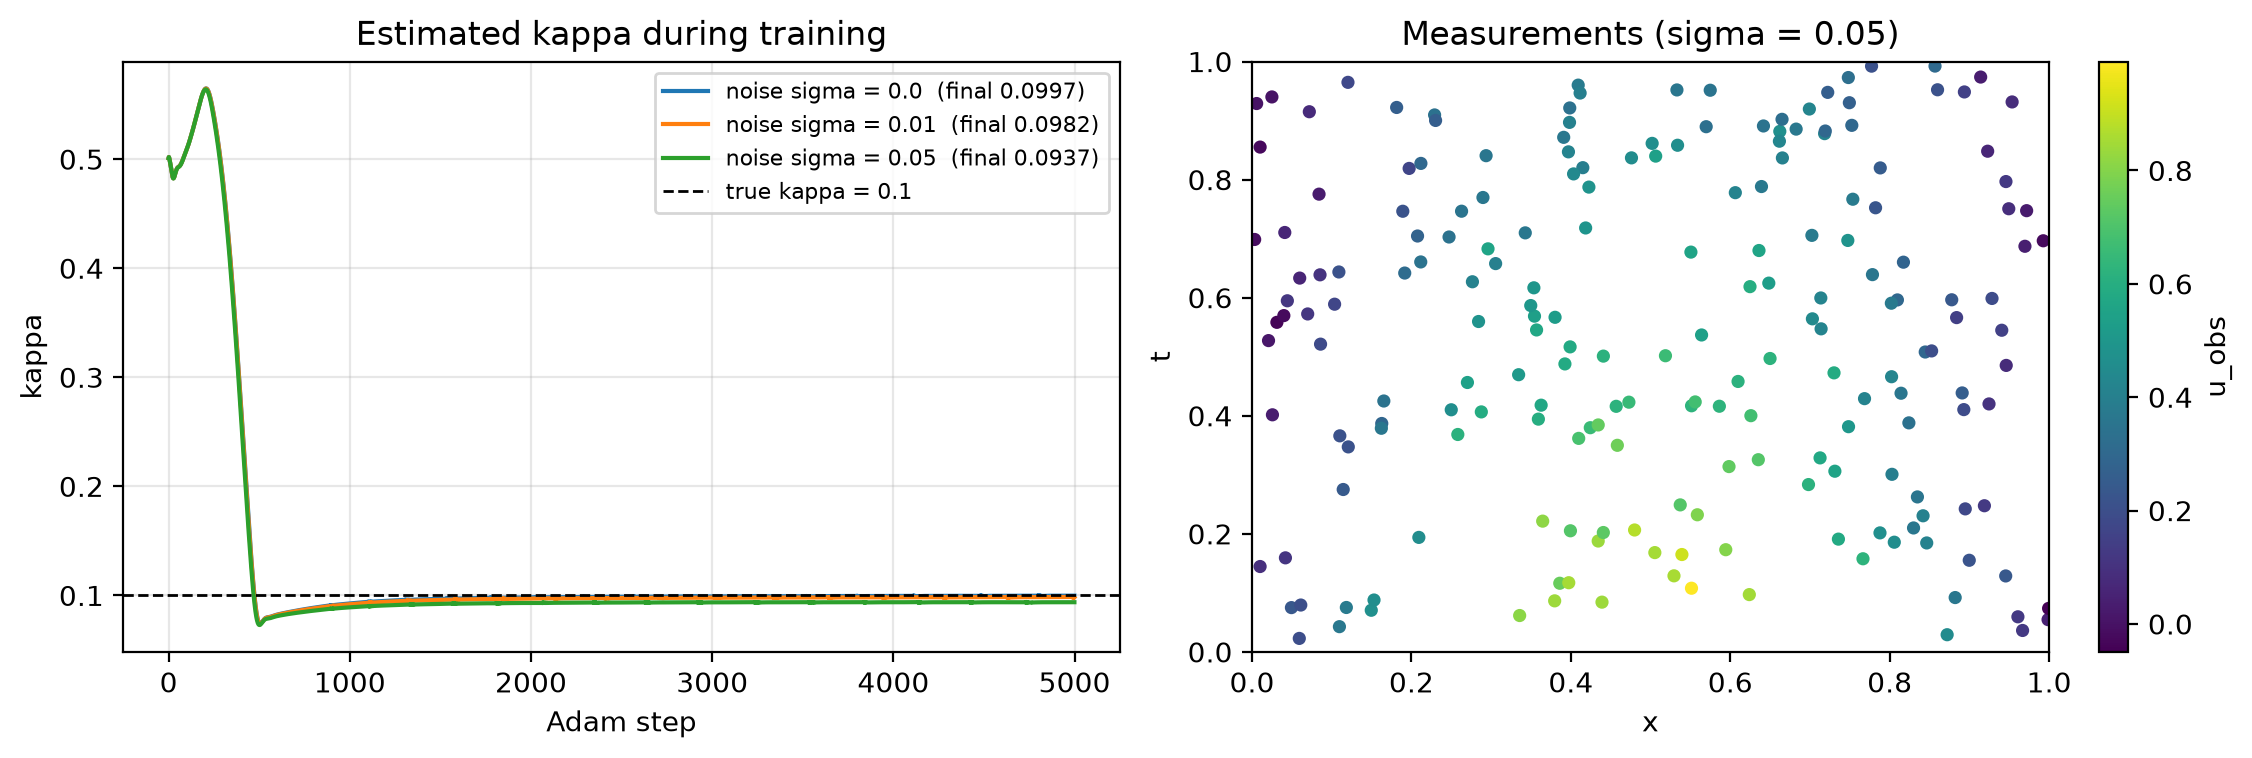
\includegraphics[width=0.74\linewidth]{figures/inverse_kappa.png}
\figcap{왼쪽: 학습 중 $\kappa$의 변화 (세 곡선이 거의 겹친다). 오른쪽: $\sigma=0.05$일 때의 측정값 $200$개.}
\vskip1mm
\begin{tabular}{@{}lccc@{}}
\toprule
잡음 $\sigma$ & $0$ & $0.01$ & $0.05$ \\
\midrule
추정한 $\kappa$ (참값 $0.1$) & $0.09975$ & $0.09822$ & $0.09375$ \\
상대오차 $|\kappa_{\text{추정}}-0.1|/0.1$ & $0.25\%$ & $1.8\%$ & $6.3\%$ \\
\bottomrule
\end{tabular}
\end{frame}

\begin{frame}{결과의 해석}
\begin{itemize}
\item $\kappa$는 처음 $200$ step 동안 $0.56$까지 오른 뒤 $300$--$500$ step 사이에 급격히 내려온다
\item 초기의 $u_\theta$는 측정값과 맞지 않으므로 그 $u_t$, $u_{xx}$로 정한 $\kappa$도 의미가 없다. \textbf{$u_\theta$가 측정값에 맞은 뒤에} $\kappa$가 수렴한다
\item 잡음이 없으면 오차 $0.25\%$, 잡음이 커질수록 오차가 커진다. 이 실험에서는 모두 참값보다 작게 추정되었다
\end{itemize}
\vskip3mm
\begin{keybox}
측정 오차가 추정값에서 증폭되는 것은 역문제의 일반적인 성질 (\textbf{ill-posedness})이며, 정칙화 등으로 다룬다.
\end{keybox}
\end{frame}

% =================================================
\section{2차원 타원형 방정식}
% =================================================

\begin{frame}{문제: 원판에서 $\nabla\cdot(\sigma\nabla u)=0$}
단위 원판 $\Omega=\{x^2+y^2<1\}$에서
\[
\nabla\cdot\big(\sigma(x,y)\,\nabla u\big)=0\quad\text{in }\Omega,\qquad u=\cos\theta\quad\text{on }\partial\Omega.
\]
\begin{itemize}
\item $\nabla\cdot(\sigma\nabla u)=(\sigma u_x)_x+(\sigma u_y)_y$. $\sigma>0$이면 \textbf{타원형}, Dirichlet 경계조건 하나로 해가 유일
\item $u$: 전위, $\sigma$: 전기전도도. 전류밀도 $-\sigma\nabla u$가 내부에서 생기거나 사라지지 않는다
\item $\sigma$: 배경값 $1$에 가우스 함수 모양의 덩어리 둘
\end{itemize}
\[
\sigma(x,y)=1+1.5\,e^{-\frac{(x-0.35)^2+(y-0.2)^2}{2\cdot0.15^2}}-0.5\,e^{-\frac{(x+0.35)^2+(y+0.25)^2}{2\cdot0.18^2}}
\]
\begin{itemize}
\item 정확한 해의 식이 없으므로 기준 해는 유한요소법 (\texttt{fem\_disk.py}, 노드 $31731$개; $\sigma=1$일 때 오차 $10^{-5}$ 정도)
\end{itemize}
\end{frame}

\begin{frame}[fragile]{residual: 발산을 자동미분으로}
입력 \texttt{X} $=(x,y)$, 모양 $(N,2)$. 자동미분 세 번:
\begin{lstlisting}
def residual(X):
    u = model(X)                                     # (N, 1)
    s = sigma(X[:, 0:1], X[:, 1:2])                  # (N, 1)
    flux = s * grad(u, X)                            # (N, 2) = sigma * (u_x, u_y)
    div = grad(flux[:, 0:1], X)[:, 0:1] + grad(flux[:, 1:2], X)[:, 1:2]   # (sigma u_x)_x + (sigma u_y)_y
    return div
\end{lstlisting}
\begin{itemize}
\item \texttt{grad(u, X)}는 $(u_x,u_y)$를 한 번에 준다
\item 플럭스의 첫 열 $\sigma u_x$의 미분에서 $x$ 열을, 둘째 열 $\sigma u_y$의 미분에서 $y$ 열을 가져와 더한다
\item $\sigma$의 도함수는 따로 계산하지 않는다: $\sigma$가 \texttt{X}로부터 계산된 텐서이므로 곱의 미분 $(\sigma u_x)_x=\sigma_xu_x+\sigma u_{xx}$를 autograd가 처리한다
\end{itemize}
\end{frame}

\begin{frame}{점과 loss}
\begin{itemize}
\item 내부 점 $20000$개를 원판에 균일하게 ($r=\sqrt{U}$, $\theta=2\pi V$), 매 step $1000$개를 미니배치로
\item 경계점 $2000$개, 매 step $256$개
\end{itemize}
\[
\loss=\frac1{1000}\sum_{i}\big(\nabla\cdot(\sigma\nabla u_\theta)\big)^2\Big|_{X_i}+10\cdot\frac1{256}\sum_k\big(u_\theta(X_k)-\cos\theta_k\big)^2
\]
\begin{itemize}
\item 신경망 $2\to64\to64\to64\to1$ ($\tanh$), Adam $5000$ step
\item 학습률은 $1667$ step마다 $0.3$배 (\texttt{torch.optim.lr\_scheduler.StepLR})
\item GPU (RTX 4070)에서 약 $110$초
\end{itemize}
\end{frame}

\begin{frame}{결과}
\small 유한요소 해의 노드 $31731$개에서 상대오차 $2.9\times10^{-3}$, 최대 절대오차 $6.3\times10^{-3}$.
\vskip1mm
\centering
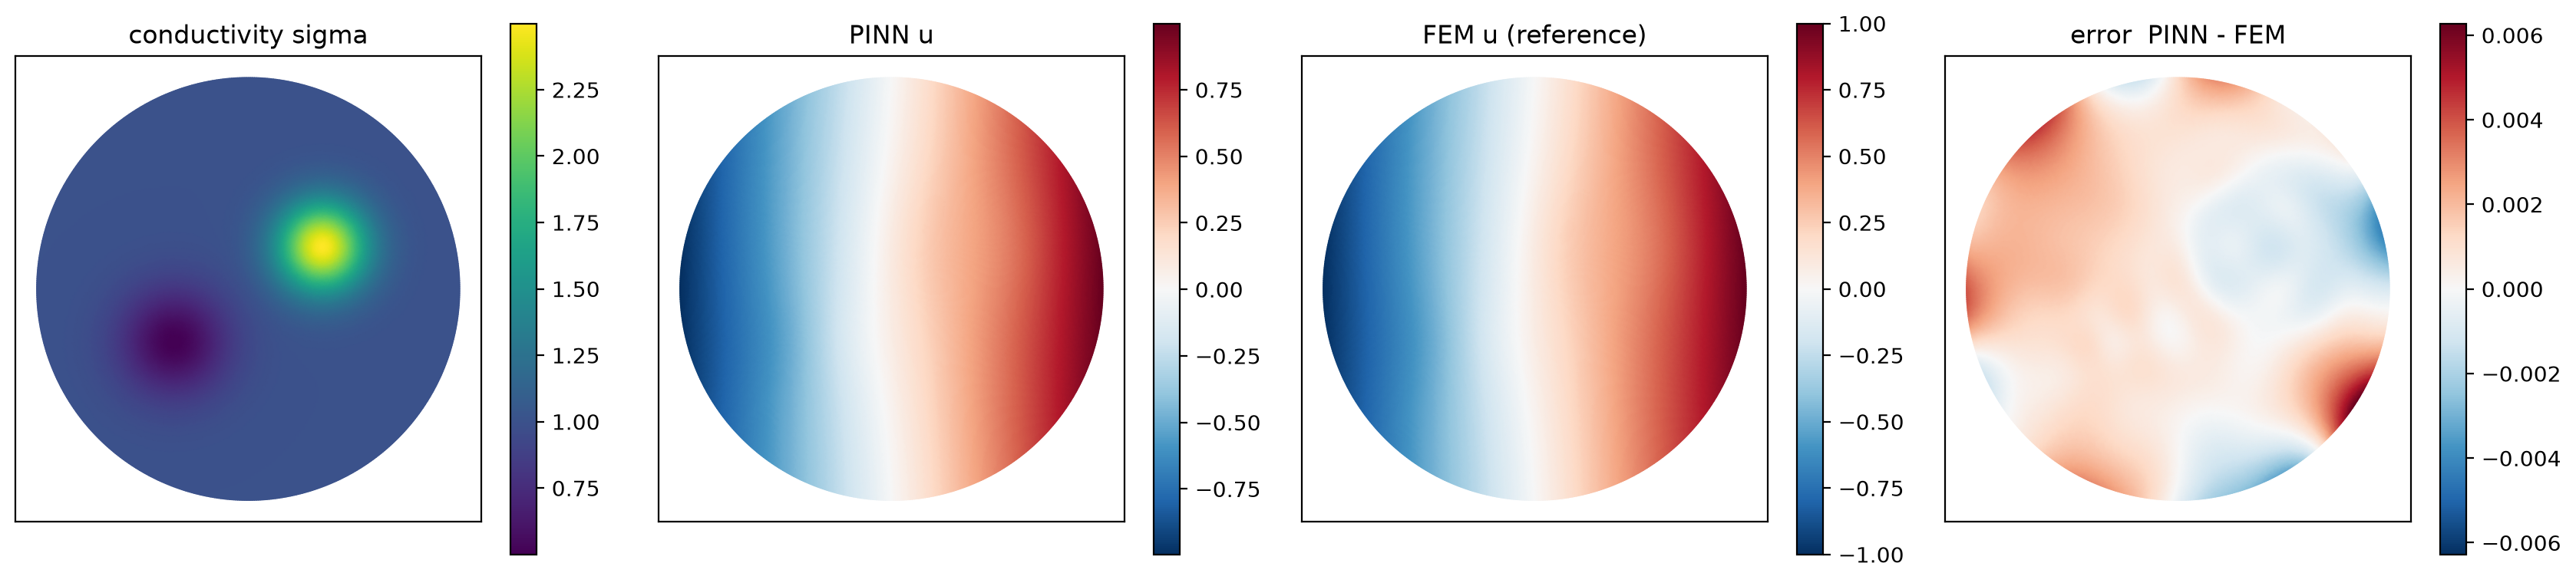
\includegraphics[width=0.96\linewidth]{figures/elliptic_field.png}
\figcap{왼쪽부터 $\sigma$, PINN의 해, 유한요소 해, 오차.}
\raggedright
\vskip1mm
\begin{itemize}
\item 등위선이 $\sigma$가 큰 곳 (오른쪽 위)에서는 벌어지고 작은 곳 (왼쪽 아래)에서는 좁아진다: 전도도가 크면 작은 전위차로도 같은 전류가 흐른다
\item 처음 PDE 항 $5\times10^{-3}$, 경계 항 $0.5$: 상수 함수는 이 방정식을 만족한다 (열 방정식과 같은 현상)
\item 오차가 가장 큰 곳은 경계 근처
\end{itemize}
\end{frame}

% =================================================
\section{역문제 2: 전기 임피던스 단층촬영 (EIT)}
% =================================================

\begin{frame}{문제: 경계의 전류와 전압으로 내부의 $\sigma$ 찾기}
이번에는 $\sigma$를 모른다. 경계에 전류 $g_j$를 흘려 넣으면 내부의 전위 $u_j$는
\[
\nabla\cdot(\sigma\nabla u_j)=0\quad\text{in }\Omega,\qquad \sigma\,\partial_nu_j=g_j\quad\text{on }\partial\Omega
\]
를 만족하고, 경계의 전압 $f_j=u_j|_{\partial\Omega}$를 측정한다 ($\partial_n$: 바깥 법선 방향 미분).
\vskip2mm
\begin{keybox}[EIT]
전류--전압 쌍 $(g_j,f_j)$ 여러 개로부터 내부의 전도도 $\sigma$를 찾는 문제
\end{keybox}
\begin{itemize}
\item 전류: $g_j=\cos n\theta,\ \sin n\theta$ ($n=1,\dots,4$), 모두 $J=8$쌍
\item 전압: 참값 $\sigma$ (앞 절의 것)로 유한요소법을 풀어 만든 $f_j$를 경계의 $4096$개 점에서. PINN은 참값 $\sigma$를 모른다
\item 전극은 따로 생각하지 않고, 경계 전체에서 전압을 측정한다고 둔다
\end{itemize}
\end{frame}

\begin{frame}{데이터 한 쌍: 중심각 $\theta$에 대한 전류와 전압}
\small 첫 번째 쌍 $j=1$: 경계에 전류 $g_1=\cos\theta$를 흘려 넣고 (입력), 경계의 전압 $f_1$을 잰다 (출력). (\texttt{eit\_boundary\_data.py})
\vskip1mm
\centering
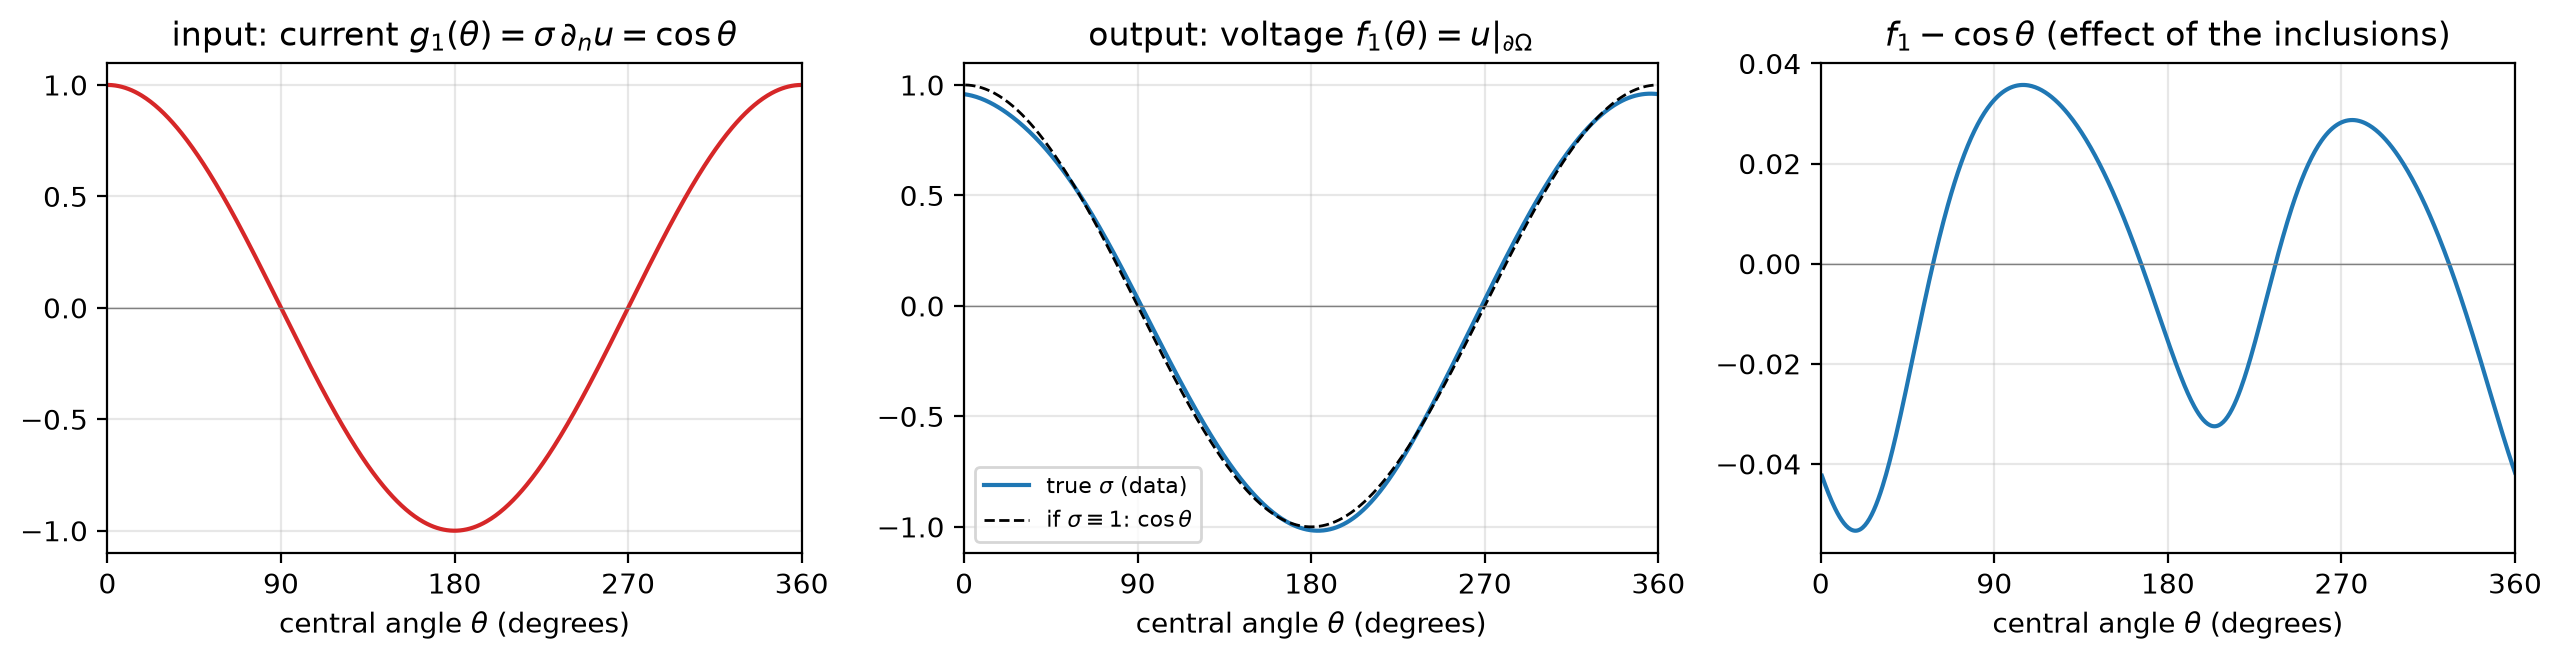
\includegraphics[width=0.96\linewidth]{figures/eit_data_theta.png}
\raggedright
\vskip1mm
\begin{itemize}
\item $\sigma\equiv1$이면 $u=r\cos\theta$이므로 전압은 정확히 $\cos\theta$ (점선)
\item 실제 전압과 $\cos\theta$의 차이는 최대 $0.053$ (약 $5\%$). 내부의 $\sigma$에 대한 정보는 \textbf{이 작은 차이}에만 들어 있다
\item 이런 쌍이 $J=8$개 ($\cos n\theta$, $\sin n\theta$, $n=1,\dots,4$). PINN이 보는 데이터는 이것이 전부이다
\end{itemize}
\end{frame}

\begin{frame}{같은 쌍을 phantom 둘레에 그리면}
\centering
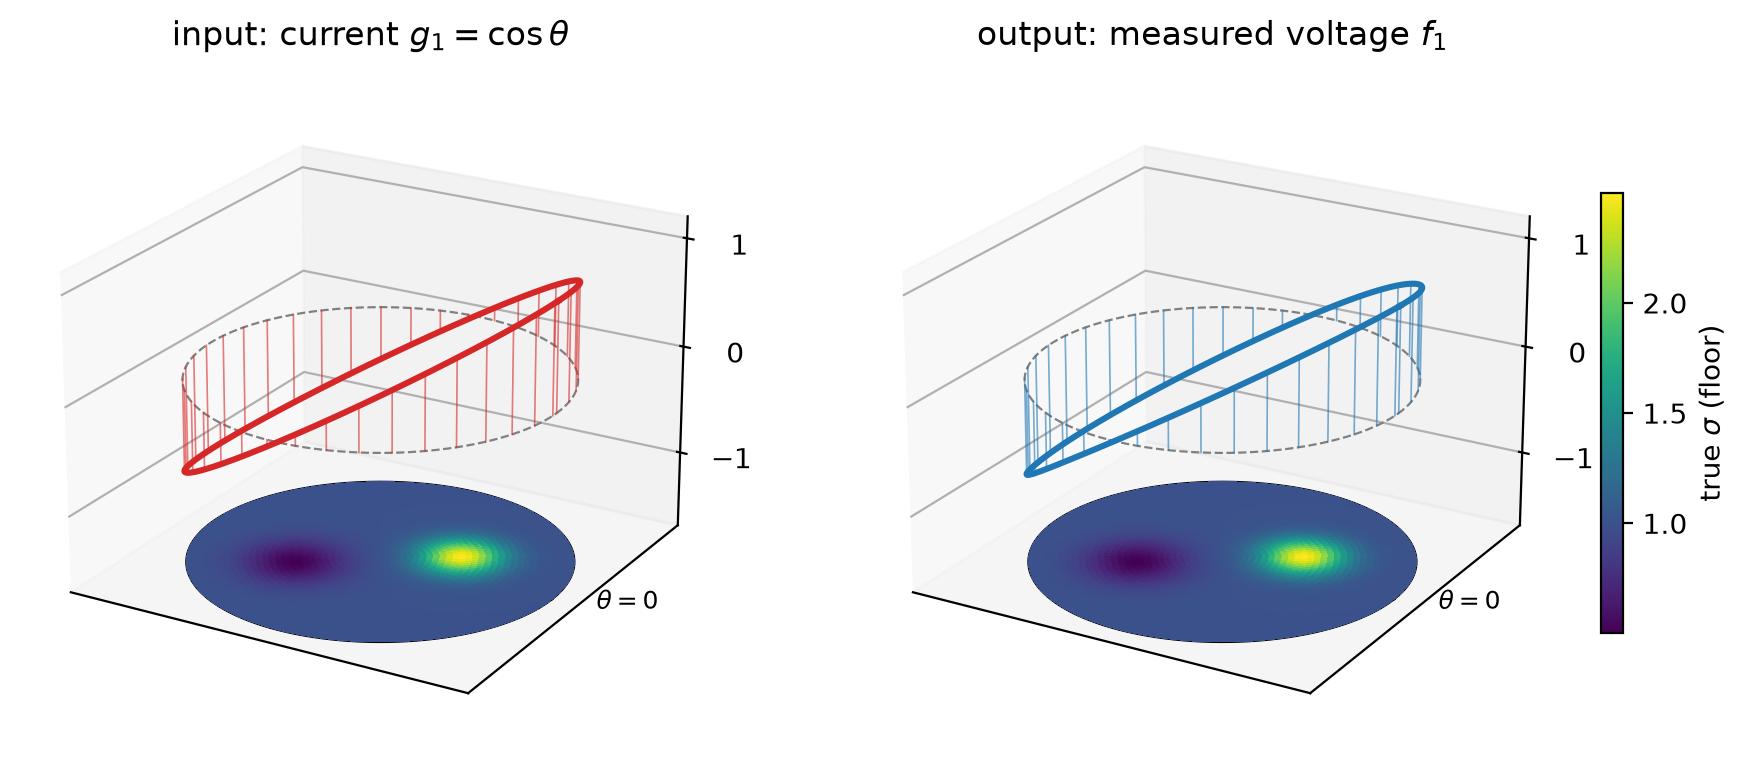
\includegraphics[width=0.8\linewidth]{figures/eit_data_3d.png}
\figcap{바닥: 참값 $\sigma$ (PINN은 모른다). 왼쪽: 원판의 둘레를 따라 흘려 넣은 전류 $g_1$. 오른쪽: 둘레에서 잰 전압 $f_1$.}
\figcap{두 곡선은 거의 같아 보인다. 경계에서 잰 값이 내부의 $\sigma$에 둔감하다는 것이 EIT가 어려운 (ill-posed) 이유이다.}
\end{frame}

\begin{frame}{두 개의 신경망}
미지수 $\sigma$와 $u_1,\dots,u_J$를 각각 신경망으로 둔다.
\[
\sigma(x,y)=s_\phi(x,y),\qquad \big(u_1,\dots,u_J\big)(x,y)=u_\theta(x,y).
\]
\begin{itemize}
\item $u_\theta$: 입력 $2$개, 출력 $J$개인 신경망 하나
\item $s_\phi$: 입력 $2$개, 출력 $1$개인 신경망
\end{itemize}
loss = 내부 residual + 경계 전압 오차 + 경계 전류 오차:
\[
\loss(\theta,\phi)=\frac1J\sum_{j}\frac1{B}\sum_i\big(\nabla\cdot(\sigma\nabla u_j)\big)^2\Big|_{X_i}
+\lambda\,\frac1J\sum_j\frac1{N_b}\sum_k\Big[\big(u_j-f_j\big)^2+\big(\sigma\,\partial_nu_j-g_j\big)^2\Big]\Big|_{X_k}
\]
역전파는 두 신경망의 매개변수 $\theta$, $\phi$ 모두에 gradient를 준다.
\end{frame}

\begin{frame}[fragile]{코드 (\texttt{pinn\_eit.py})}
\begin{lstlisting}
def loss_terms():
    X = X_f[torch.randint(0, N_f, (batch,), device=device)].clone().requires_grad_(True)
    U, S = u_net(X), s_net(X)
    loss_pde = 0.0
    for j in range(J):
        flux = S * grad(U[:, j:j+1], X)
        div = grad(flux[:, 0:1], X)[:, 0:1] + grad(flux[:, 1:2], X)[:, 1:2]
        loss_pde = loss_pde + torch.mean(div**2) / J
    Xb = X_b.clone().requires_grad_(True)
    Ub, Sb = u_net(Xb), s_net(Xb)
    dudn = torch.cat([(grad(Ub[:, j:j+1], Xb) * Xb).sum(dim=1, keepdim=True)
                      for j in range(J)], dim=1)
    loss_D = torch.mean((Ub - f_b)**2)            # voltage data
    loss_N = torch.mean((Sb * dudn - g_b)**2)     # current data
    return loss_pde, loss_D, loss_N
\end{lstlisting}
\begin{itemize}
\item residual은 앞 절과 같은 계산을 $J$번
\item 원판의 경계에서 바깥 법선은 위치 벡터 $(x,y)$ 자체: $\partial_nu=\nabla u\cdot(x,y)$ $\Rightarrow$ \texttt{(grad(...) * Xb).sum(1)}
\end{itemize}
\end{frame}

\begin{frame}{설정과 오차의 정의}
$\sigma$의 오차는 상대 $L^2$ 오차에서 분모만 바꾼
\[
\frac{\|s_\phi-\sigma\|_2}{\|\sigma-1\|_2}
\]
로 잰다 (시험점: $[-1,1]^2$의 $101\times101$ 격자 중 원판 안의 점). 경계 데이터를 쓰지 않고 $\sigma\equiv1$로 답하면 $1$.
\vskip2mm
\begin{center}
\small
\begin{tabular}{@{}ll@{}}
\toprule
전류--전압 쌍 & $J=8$ \\
경계점 / 내부 collocation point & $N_b=4096$ / $N_f=20000$ (매 step $2000$개 미니배치) \\
loss 가중치 & $\lambda=100$ \\
신경망 & $u_\theta$ 은닉층 $4$개, $s_\phi$ 은닉층 $3$개, 폭 $64$, $\tanh$ \\
학습 & Adam $150000$ step, 학습률 $10^{-3}$에서 $50000$ step마다 $0.3$배 \\
시간 & GPU (RTX 4070)에서 약 $3.8$시간 \\
\bottomrule
\end{tabular}
\end{center}
\end{frame}

\begin{frame}{결과: 상대오차 $0.573$}
\centering
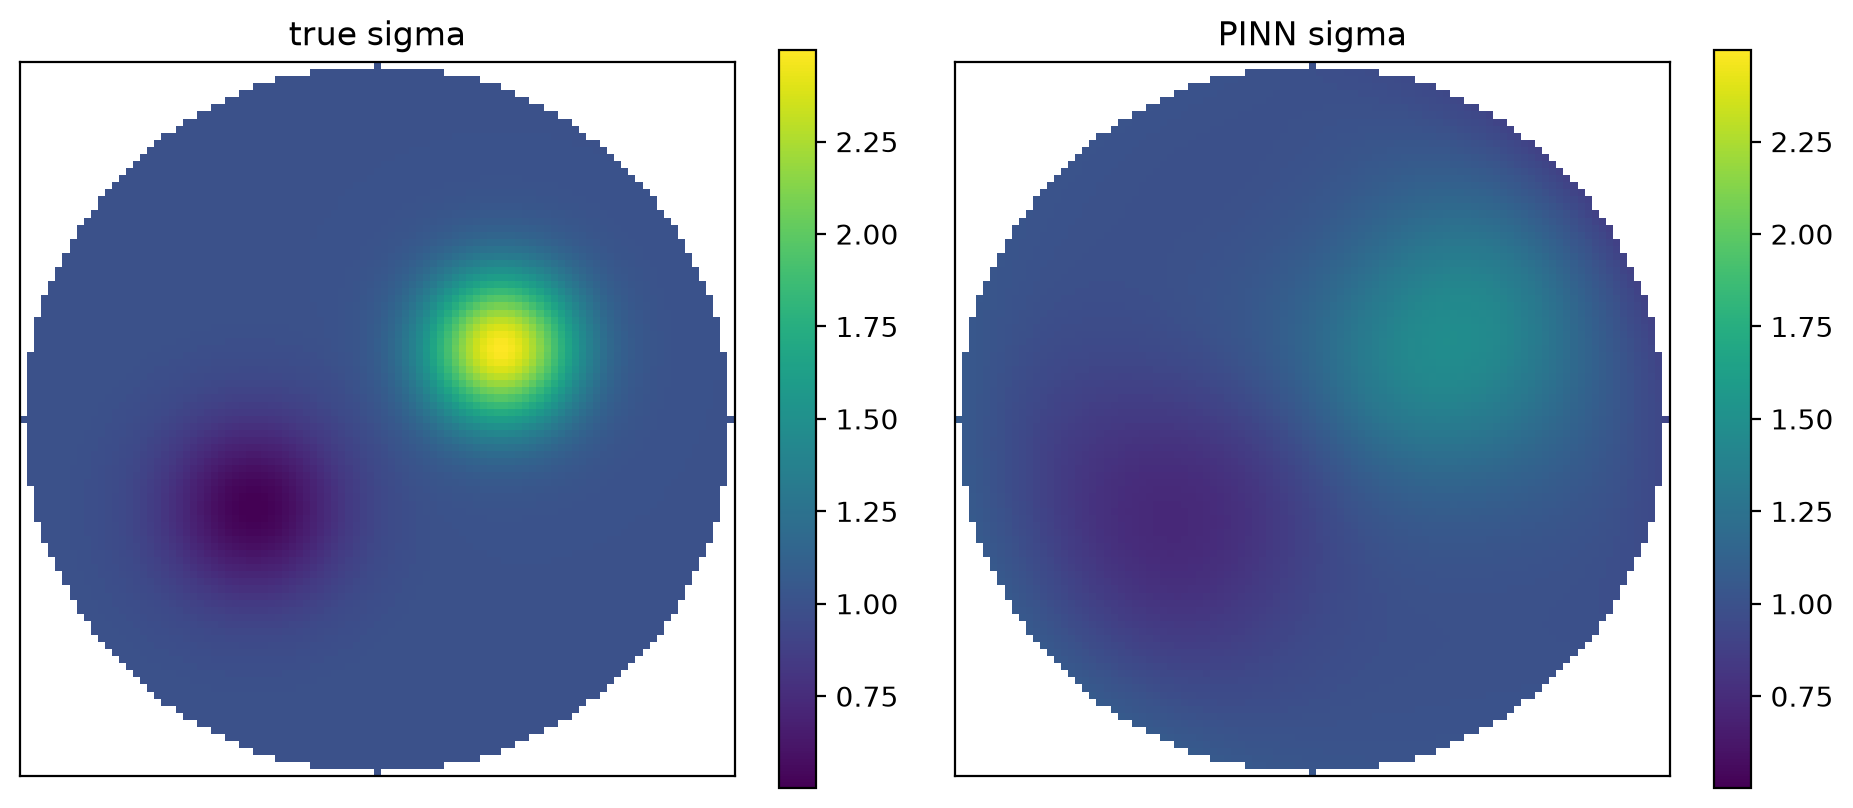
\includegraphics[width=0.8\linewidth]{figures/eit_sigma.png}
\figcap{왼쪽: 참값 $\sigma$. 오른쪽: 경계의 전류--전압 쌍 $8$개에서 복원한 $\sigma=s_\phi$. 색의 범위는 같다.}
\figcap{복원한 $\sigma$의 범위 $[0.73,\,1.48]$ (참값 $[0.50,\,2.50]$).}
\end{frame}

\begin{frame}{loss는 작은데 $\sigma$의 오차는 크다}
\begin{columns}[c,onlytextwidth]
\begin{column}{0.5\textwidth}
\centering
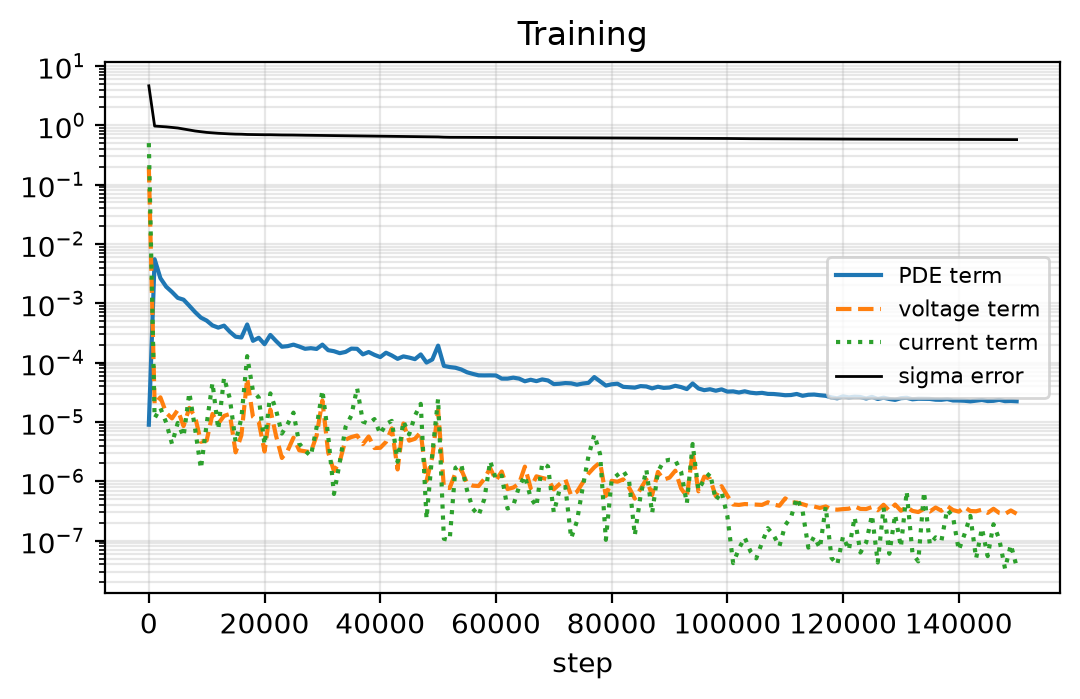
\includegraphics[width=0.8\linewidth]{figures/eit_loss.png}
\figcap{loss의 세 항과 $\sigma$의 상대오차.}
\end{column}
\begin{column}{0.48\textwidth}
\small
\begin{itemize}
\item $\sigma>1$인 덩어리와 $\sigma<1$인 덩어리의 \textbf{위치}를 찾았다. $\sigma$의 값을 직접 알려 준 적은 없다
\item 복원한 덩어리는 넓게 퍼져 있고 진폭이 작다
\item 마지막 step: PDE $2.2\times10^{-5}$, 전압 $2.8\times10^{-7}$, 전류 $3.7\times10^{-8}$
\item 경계 측정값을 거의 맞추어도 내부의 $\sigma$는 부정확: EIT는 \textbf{ill-posed} 문제
\end{itemize}
\end{column}
\end{columns}
\vskip2mm
\begin{remarkbox}[학습에 영향을 주는 것들: 여러 값을 시험해 보아야 한다]
\footnotesize 전류--전압 쌍의 수, 경계점과 collocation point의 수, 미니배치 크기 $\cdot$ loss 가중치 $\lambda$ $\cdot$ step 수, 학습률 schedule, 두 신경망의 크기 $\cdot$ 경계 데이터의 잡음
\end{remarkbox}
\end{frame}

% =================================================
\section{PINN의 한계와 요령}
% =================================================

\begin{frame}{높은 주파수의 해 (\texttt{pinn\_frequency.py})}
\small Poisson 문제와 같은 신경망, 같은 점 $64$개, 같은 Adam $5000$ step으로
$\ -u''=(k\pi)^2\sin(k\pi x)$, $u(0)=u(1)=0$, $k=1,2,4,8$ (정확한 해 $\sin(k\pi x)$; residual을 $(k\pi)^2$로 나눔).
\vskip1mm
\centering
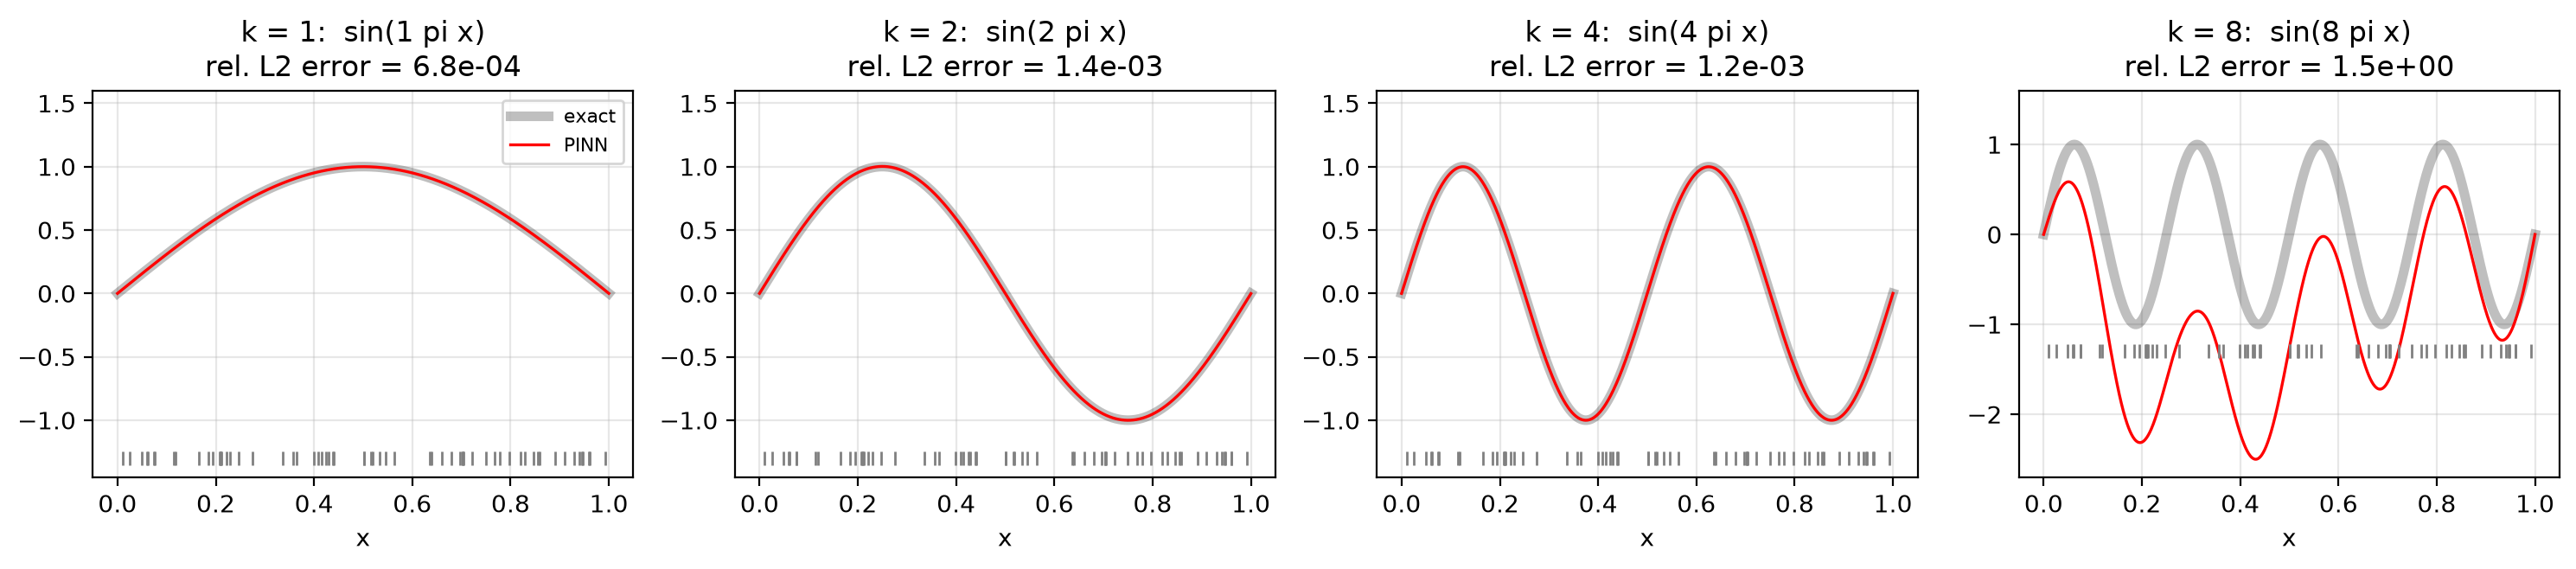
\includegraphics[width=\linewidth]{figures/frequency.png}
\figcap{같은 조건으로 학습하면 $k=8$에서 실패한다 (마지막 그림은 세로축 범위가 다르다).}
\vskip1mm
\begin{tabular}{@{}lcccc@{}}
\toprule
$k$ & $1$ & $2$ & $4$ & $8$ \\
\midrule
마지막 loss (나눈 뒤) & $4.1\times10^{-6}$ & $3.2\times10^{-6}$ & $8.7\times10^{-6}$ & $4.5\times10^{-4}$ \\
상대오차 & $6.8\times10^{-4}$ & $1.5\times10^{-3}$ & $1.2\times10^{-3}$ & $1.5$ \\
\bottomrule
\end{tabular}
\end{frame}

\begin{frame}{$k=8$: 원인은 collocation point에 대한 과적합}
\small residual을 학습에 쓴 점 (훈련)과 $1001$개 격자점 (테스트)에서 따로 잰다. 조건마다 seed $3$개.
\vskip1mm
\centering
\footnotesize
\begin{tabular}{@{}llccc@{}}
\toprule
조건 & seed & 훈련 residual$^2$ & 테스트 residual$^2$ & 상대오차 \\
\midrule
점 $64$개, $5000$ step & $0$ & $4.5\times10^{-4}$ & $3.8\times10^{-3}$ & $1.5$ \\
 & $1$ & $1.4\times10^{-1}$ & $2.5\times10^{-1}$ & $10$ \\
 & $2$ & $1.1\times10^{-2}$ & $3.3\times10^{-2}$ & $7.9$ \\
\midrule
점 $64$개, $20000$ step & $0$ & $8.3\times10^{-6}$ & $2.7\times10^{-4}$ & $0.39$ \\
 & $1$ & $1.6\times10^{-3}$ & $1.0\times10^{-1}$ & $4.5$ \\
 & $2$ & $2.0\times10^{-5}$ & $6.5\times10^{-3}$ & $1.7$ \\
\midrule
점 $10000$개 (미니배치 $256$), & $0$ & $5.8\times10^{-5}$ & $6.1\times10^{-5}$ & $0.0076$ \\
$20000$ step & $1$ & $1.4\times10^{-5}$ & $1.4\times10^{-5}$ & $0.015$ \\
 & $2$ & $2.6\times10^{-6}$ & $2.7\times10^{-6}$ & $0.027$ \\
\bottomrule
\end{tabular}
\raggedright
\small
\begin{itemize}
\item 점 $64$개: 훈련 residual $<$ 테스트 residual, 오래 학습할수록 차이가 커진다 ($2$--$8$배 $\to$ $30$--$300$배)
\item 점 $10000$개: 훈련과 테스트 residual이 같고 상대오차 $0.008$--$0.03$
\end{itemize}
\end{frame}

\begin{frame}{점을 충분히 만들어 두고 미니배치로 오래 학습한다}
\centering
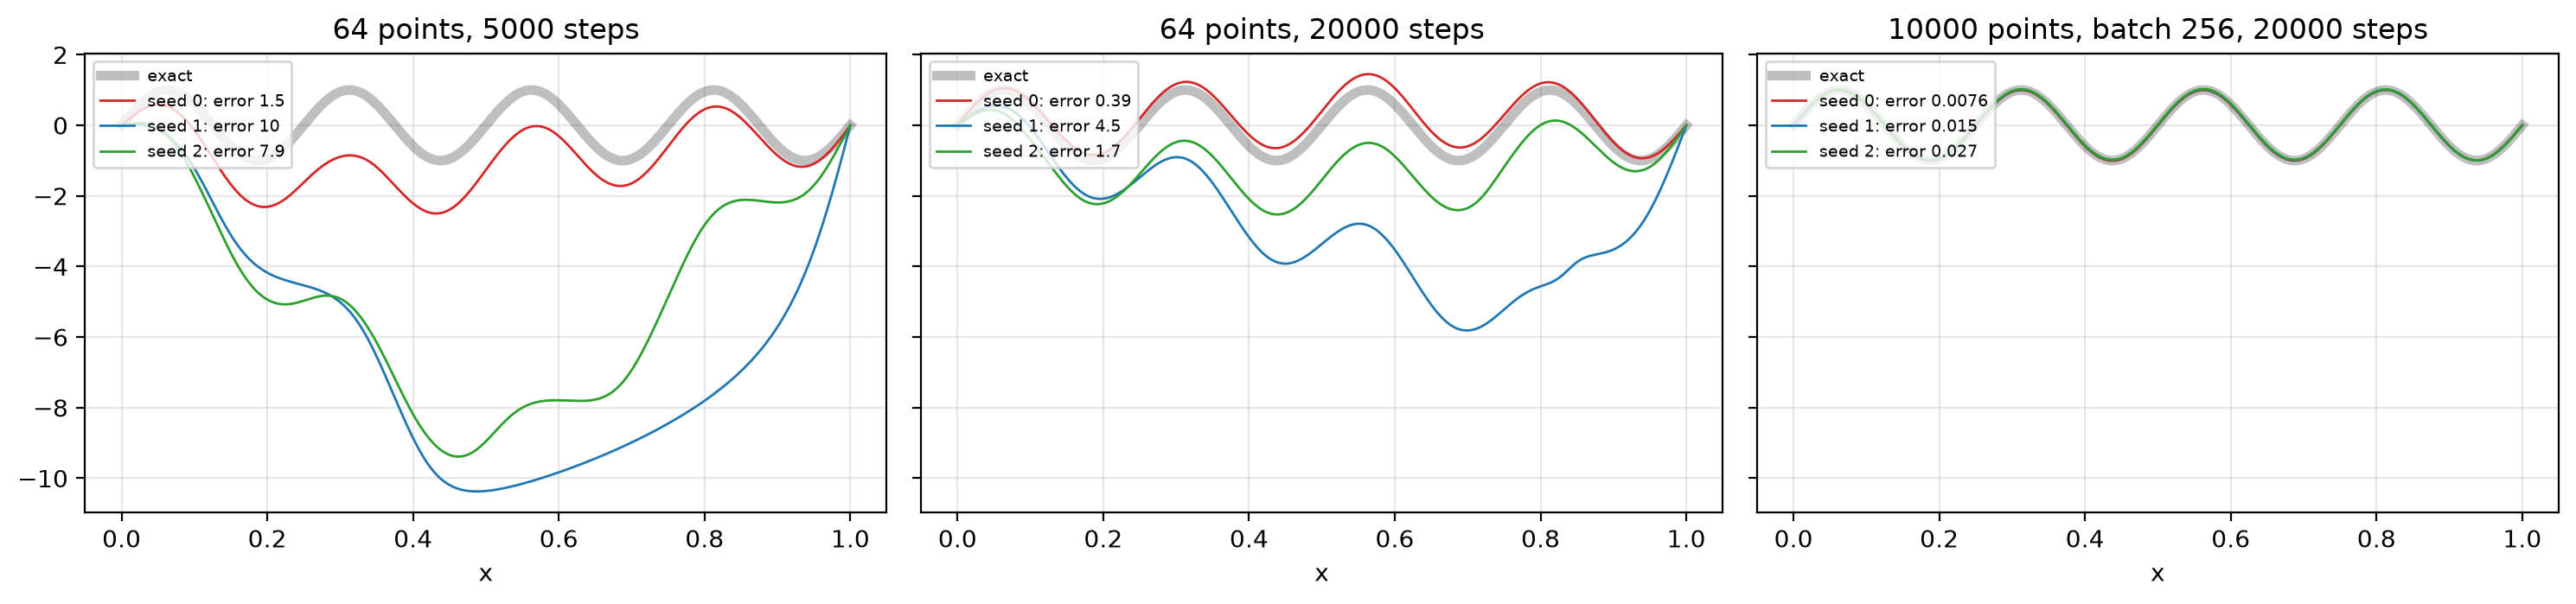
\includegraphics[width=0.94\linewidth]{figures/frequency_k8.png}
\figcap{$k=8$의 세 조건. 각 그림에 seed $3$개의 결과를 겹쳐 그렸다.}
\raggedright
\small
\begin{itemize}
\item 해가 빠르게 진동할수록 방정식을 만족해야 할 정보가 많으므로 점이 더 많이 필요하다
\item 신경망은 낮은 주파수 성분을 먼저 학습하는 경향 (\textbf{spectral bias})이 있어, 높은 주파수의 해에는 step도 더 많이 필요하다
\item collocation point는 계산으로 얼마든지 만들 수 있다: 지도학습과 달리 훈련 데이터의 양에 제한이 없다
\item 그 밖의 방법: Fourier feature $\big(\sin(2\pi\omega_jx),\cos(2\pi\omega_jx)\big)_j$, 영역을 나누어 작은 신경망 여러 개
\end{itemize}
\end{frame}

\begin{frame}{loss 항의 균형}
PINN의 loss는 성격이 다른 항의 가중합이다.
\vskip2mm
\begin{itemize}
\item Poisson 문제의 처음 loss: PDE 항 $46$, 경계 항 $0.03$
\item 크기가 크게 다르면 gradient가 큰 항만 줄어든다
\item $\lambda$를 조절하거나, 학습 중 각 항의 gradient 크기에 따라 가중치를 자동으로 바꾼다
\item 적절한 가중치는 문제마다 다르다
\end{itemize}
\end{frame}

\begin{frame}{고전적인 수치해법과 비교하면}
같은 Poisson 문제를 \textbf{유한차분법}으로: $u''(x_i)\approx(u_{i-1}-2u_i+u_{i+1})/\Delta x^2$ $\Rightarrow$ 연립일차방정식 하나.
\vskip1mm
\begin{remarkbox}[수치해법으로서의 PINN]
\small
두 방법 모두 해를 유한 개의 미지수로 표현하고, 방정식을 유한 개의 점에서 만족시킨다.
\begin{itemize}
\item 유한차분법: 미지수는 격자점의 값, 도함수는 차분으로 근사, 선형 방정식 $\Rightarrow$ $A\vect u=\vect b$
\item PINN: 미지수는 $\theta$, 도함수는 자동미분으로 정확히, residual을 최소제곱으로 줄인다. $u_\theta$는 $\theta$에 대해 비선형 $\Rightarrow$ 비볼록 최적화
\end{itemize}
\end{remarkbox}
\begin{center}
\small
\begin{tabular}{@{}lcc@{}}
\toprule
방법 & 상대오차 & 시간 \\
\midrule
유한차분법 (구간 $100$개, CPU) & $8.2\times10^{-5}$ & 약 $1$--$10$ ms \\
PINN (Adam $5000$ step, GPU) & $6.1\times10^{-5}$ & 약 $40$ s \\
PINN (Adam $5000$ step + L-BFGS, GPU) & $1.5\times10^{-5}$ & 약 $40$ s \\
\bottomrule
\end{tabular}
\end{center}
\end{frame}

\begin{frame}{PINN은 언제 쓰는가}
순문제에서 PINN은 유한차분법, 유한요소법보다 \textbf{수천 배 느리고} 오차에 대한 이론적 보장도 약하다.
\begin{keybox}[PINN이 유리한 경우]
\begin{itemize}
\item \textbf{역문제}와 데이터 동화: 측정값과 방정식을 하나의 loss로. 코드는 순문제와 거의 같다
\item \textbf{격자가 필요 없다}: 복잡한 영역이나 고차원 문제에 적용하기 쉽다
\item 방정식의 일부만 알거나 데이터가 흩어져 있는 경우
\end{itemize}
\end{keybox}
\begin{remarkbox}[더 나아가: 연산자를 배우기]
\footnotesize PINN은 $f$, $\kappa$가 바뀌면 다시 학습해야 한다. 해 연산자 $f\mapsto u$를 근사하는 DeepONet (2021), FNO (2021)는 학습 후 새로운 $f$의 해를 forward 한 번으로 얻는다.
\end{remarkbox}
\end{frame}

% =================================================
\section{정리}
% =================================================

\begin{frame}{PINN: 정리 (1)}
\begin{keybox}[정리]
\begin{itemize}
\item PINN은 신경망 $u_\theta$의 residual (방정식을 어기는 정도)과 초기/경계조건 오차를 loss로 하여 미분방정식을 푼다
\item 입력에 대한 미분 $u_x$, $u_{xx}$는 \texttt{autograd.grad(..., grad\_outputs=ones\_like(u), create\_graph=True)}로 구한다.
이 계산은 원래 그래프에 매달린 미분 그래프를 만들며, residual이 둘을 하나의 그래프로 잇는다
\item \texttt{loss.backward()}는 합쳐진 그래프를 거꾸로 지나며, 한 가중치에서 출발한 여러 경로의 기여를 \textbf{더한다}.
optimizer는 이 사실을 모르고 \texttt{.grad}만 쓴다
\item 입력이 여러 개이면 \texttt{grad}의 결과에서 필요한 열을 잘라 쓴다. 모양 $(N,1)$을 유지하자
\end{itemize}
\end{keybox}
\end{frame}

\begin{frame}{PINN: 정리 (2)}
\begin{keybox}[정리]
\begin{itemize}
\item 역문제에서는 미지의 계수를 \texttt{nn.Parameter}로 두고 측정값 항과 방정식 항을 함께 최소화한다.
미지의 계수가 함수이면 ($\sigma(x,y)$, EIT) 그것도 신경망으로 둔다
\item 해가 빠르게 진동할수록 collocation point가 많이 필요하다. 점이 적으면 점에서만 방정식을 만족하는 과적합이 일어난다.
점을 충분히 만들어 두고 미니배치로 오래 학습한다
\item 한계: loss 항의 균형, 계산 비용. 순문제에서는 고전적인 수치해법이 훨씬 빠르다
\item PINN의 강점은 역문제, 데이터와 방정식의 결합, 격자가 필요 없다는 점이다
\end{itemize}
\end{keybox}
\end{frame}

% =================================================
\section{연습문제}
% =================================================

\begin{frame}{연습문제 (1)}
\small
\begin{enumerate}
\item 가장 작은 신경망에서 $x=0$일 때 $a$, $h$, $u$, $u_x$, $u_{xx}$를 손으로 계산하라 ($\tanh(-0.2)\approx-0.19738$).
\texttt{autograd\_tiny.py}의 \texttt{x}를 바꾸어 확인하라.
\item 역전파 그래프에서 $\partial\loss/\partial b_2$의 경로가 하나뿐인 이유를 설명하라.
$r=u_{xx}$ ($u''=0$의 residual)로 loss를 만들었다면 $\partial\loss/\partial b_2$는 얼마인가? 이것이 Poisson 문제에서 경계 항이 필요한 이유와 어떻게 관련되는가?
\item \texttt{pinn\_poisson\_1d.py}의 \texttt{derivative} 함수에서 \texttt{create\_graph=True}를 지우고 실행해 보라.
어떤 오류가 어느 줄에서 나는가? 첫 번째 \texttt{derivative} 호출에서만 지우면?
\item \texttt{nn.Tanh()}를 \texttt{nn.ReLU()}로 바꾸어 학습시켜라. 오류가 나는가? loss와 상대오차는?
\end{enumerate}
\end{frame}

\begin{frame}{연습문제 (2)}
\small
\begin{enumerate}
\setcounter{enumi}{4}
\item 경계 항의 가중치 \texttt{lam\_b}를 $0$, $0.01$, $1$, $100$으로 바꾸어 상대오차를 비교하라.
$\lambda=0$일 때 얻은 해는 어떤 모양인가? 그 해도 $-u''=f$는 만족하는가?
\item collocation point를 \textbf{매 step 새로 뽑도록} 고쳐라 (\texttt{requires\_grad\_}도 잊지 말자). residual 그림 (d)가 어떻게 바뀌는가?
\item \texttt{pinn\_heat\_1d.py}에서 $\kappa=0.5$로 바꾸어 풀어라 (정확한 해의 식도 바뀐다).
$t=1$에서의 해의 크기는 얼마여야 하는가? PINN의 결과와 비교하라.
\item \texttt{pinn\_inverse\_heat.py}에서 \texttt{N\_d}를 $200$에서 $20$, $50$으로 줄여 $\kappa$의 추정값을 비교하라.
측정값을 모두 $t<0.1$에서만 얻는다면? 예상한 뒤 실험으로 확인하라.
\item (생각해 보기) 측정값이 모두 $x=0.5$ 근처 한 점에서만 얻어졌다면 $\kappa$를 정할 수 있을까?
정확한 해 $e^{-\kappa\pi^2t}\sin(\pi x)$를 이용해 생각해 보라.
\end{enumerate}
\end{frame}

\end{document}
